\documentclass[conference]{IEEEtran}
\IEEEoverridecommandlockouts
% The preceding line is only needed to identify funding in the first footnote. If that is unneeded, please comment it out.
\usepackage[numbers]{natbib}
\usepackage{amsmath,amssymb,amsfonts}
\usepackage{algorithmic}
\usepackage{subcaption}
\usepackage{graphicx}
\usepackage{textcomp}
\usepackage{xcolor}
\def\BibTeX{{\rm B\kern-.05em{\sc i\kern-.025em b}\kern-.08em
    T\kern-.1667em\lower.7ex\hbox{E}\kern-.125emX}}
\begin{document}

\title{Availability Evaluation Models for Unmanned Aerial Vehicles (UAVs): An Analytical and a Numerical Method\\

\thanks{Identify applicable funding agency here. If none, delete this.}
}

\author{\IEEEauthorblockN{1\textsuperscript{st} Luan Lins}
\IEEEauthorblockA{\textit{Centro de Informática} \\
\textit{Universidade Federal de Pernambuco}\\
Recife-PE, Brazil \\
lcsl2@cin.ufpe.br}
\and
\IEEEauthorblockN{2\textsuperscript{nd} Paulo Maciel}
\IEEEauthorblockA{\textit{Centro de Informática} \\
\textit{Universidade Federal de Pernambuco}\\
Recife-PE, Brazil \\
prrm@cin.ufpe.br}}

\maketitle

\begin{abstract}
%The reliability and availability evaluation of unmanned aerial vehicles (UAVs) is essential, especially when these are used to save lives. However, the infrastructure planning of the UAVs is not an easy task. Thus, the hierarchical modeling strategy may guide designers to evaluate and compare some results with already implemented proposals. This paper proposes a methodology and models to evaluate the availability of critical systems implemented in unmanned aerial vehicles. Two models are proposed: The first is an analytical model to evaluate availability metrics in the primary operating mode. The second model is a numerical method model with Petri nets to use redundancy mechanisms when improving the primary operational mode no longer has as much impact. The validation of the models takes place by comparing the results obtained with the real system using different scenarios. In this work, we present three case studies showing the use of the suggested technique to evaluate a UAV flight system, given the improvements and models used. The results show that it is possible to have an availability increase of 164.71\% in each technique and 193.82\% in mixed-use.

The reliability and availability evaluation of unmanned aerial vehicles (UAVs) is essential, especially when these are used to save lives. However, the infrastructure planning of the UAVs is not easy since they have small components and limited use time. This paper proposes a methodology and models to evaluate the availability of critical systems implemented in unmanned aerial vehicles represented by Stochastic Petri Nets and Markov chains models. These UAVs follow the basic systems with one running drone and one spare drone. Thus, the hierarchical modeling strategy may guide designers to evaluate and compare some results with already implemented proposals. Closed-form equations for steady-state availability are presented, allowing direct analytical solutions for large systems. The availability equations are symbolically differentiated, allowing parametric sensitivity analysis. The results from sensitivity analysis enable system planning for improving steady-state availability. In this work, we present three case studies showing the use of the suggested technique to evaluate a UAV flight system, given the improvements and models used. The results show that it is possible to have an availability increase of 2.6x in each technique and almost 3x in mixed-use.
\end{abstract}

\begin{IEEEkeywords}
Modeling and Availability; Continuous Time Markov Chain; Stochastic Petri Net; Unmanned Aerial Vehicle (UAV);
\end{IEEEkeywords}

\section{Introduction}\label{sec:introduction}

The Internet of Things has been growing in recent years, increasing the number of connected devices around us. The global Internet of Things (IoT) market is estimated to grow from US \$800.00 billion by 2023 to US \$ 8,131.00 billion in 2030 at a compound annual growth rate (CAGR) of 20\% \citep{al2020internet}.

These devices constantly communicate and collect data that are analyzed and transformed into relevant information for decision-making that improves processes and people's quality of life. Some of these devices include smart home appliances, wearable devices, self-driving cars, industrial sensors, and drones, also called unmanned aerial vehicles (UAV), which were initially designed for direct combat. Enormous in size, UAVs were augmented with bombs and guided by remote control into enemy lines.

However, in recent years, the popularity of unmanned aerial vehicles has increased enormously now due to their ability to move autonomously, reduced structure, and applications in various domains. UAVs have been increasingly used in a wide range of applications beyond the war industry, such as surveillance \citep{basilico2015deploying}, smart agriculture \citep{lottes2017uav}, photogrammetry \citep{cesetti2011visual}, disaster management, civil security \citep {maza2011experimental}, forest fire tracking \citep{pham2017distributed}, cloud monitoring \citep{renzaglia2016monitoring}, structure supervision \citep{guerrero2013uav}, and power line inspection \citep{chang2017development}.

A percentage of UAVs also work with critical systems such as fire monitoring systems, air defence operations, and systems where continuous flights are required to maintain high monitoring availability, as they involve security, and failure could cause physical, personal, or financial damage. Therefore, there is a need for good planning of these systems where it is possible to guarantee their efficiency.

%This article compares some availability criteria for critical systems implemented in unmanned aerial vehicles to support the planning and dimensioning of these systems. We propose an analytical model to evaluate availability metrics in the primary operating mode and a numerical method model with Petri nets to use redundancy mechanisms when improving the primary operating mode no longer has as much impact. We evaluated both scenarios based on sensitivity analysis to determine the best approach for the desired level of availability. 

Some works have studied the availability of UAVs systems from the perspective of some operational modes in particular. \citet{Zaitseva2020, rusnak2019reliability} proposed a mathematical representation based on structure function and reliability block diagrams (RBD's) of a fleet of UAVs and calculated their availability and reliability according to the failure time of the device and its control unit. \citet{Machida2021, Report} performed a trade-off analysis between availability, performance, and energy consumption in image processing using the fog computing paradigm (computed on a machine connected to a network close to the device) and edge (computed on the device). \citet{Maccarthy2019} developed a stochastic analytical model for UAV system availability with cold-standby redundancy K-out-of-N. Although these works have addressed the availability of systems that use UAVs, most of them only address macro aspects of the availability of these systems, using simple modeling approaches. Unlike these works, we contemplated more detailed characteristics of the operation with UAVs, modeling the dependencies between the components and their background system.

As contributions to this work, we can list:
\begin{enumerate}
     \item Availability models for system provisioning UAVs with component improvements and redundancy mechanisms.
     \item Sensitivity analysis assessment to identify components with the greatest negative influence on availability.
     \item Three case studies assess the impacts of improving components and adding redundancy on availability.
\end{enumerate}

This article is structured as follows. Section \ref{sec:related_works} describes more recent work related to ours. Section \ref{sec:background} contains details on the concepts of evaluation and performance, Markov chains, Petri nets, and sensitivity analysis used in this study. Section \ref{sec:methodology} describes the methodology we used to carry out this study and the environment developed for the experiment. Analytical and numerical availability models are presented in detail in the \ref{sec:model} section. Section \ref{sec:case_studies} presents case studies. Finally, in the \ref{sec:conclusions} section, some conclusions are drawn from the article, and some directions for future work are discussed.


\section{Related works}\label{sec:related_works}

In the last years, some authors have worked on unmanned aerial vehicles' system availability. \citet{Petritoli2017, Petritoli2018}, provide new ideas to increase the reliability of a UAV by optimizing maintenance activities. For this, the reliability percentages assigned to each UAV system and subsystem are tracked to optimize time intervals and maintenance costs. Redundancy mechanisms and availability models are not proposed.

\citet{Zaitseva2020, rusnak2019reliability}, propose a mathematical representation of a fleet of UAVs that is based on the application of the structure-function of the system; this structure-function can be interpreted as a logical function. Although availability, reliability, and critical states of the system are considered, this study deals with the modeling of a fleet of UAVs using reliability block diagrams as a basis and does not cover aspects of UAV operation in particular, such as battery discharge, Spare UAVs and batteries and changeover time between a failed UAV and a ready-to-operate UAV.

In \citet{Machida2021, Report}, the authors performed a comprehensive analysis of the trade-off between availability, performance, and power consumption of a drone image processing system based on three different computing modes. Single drone computing mode, fog offloading, and load balancing with another drone. The authors calculated the availability of the smart drone system based on a stochastic Petri net model. Although the authors use stochastic Petri nets to evaluate metrics such as availability and performance, in this study, the authors only focus on computational processes and network link failures, where the failure of the process can be caused by software defects or any errors in the configurations. . Therefore, the authors do not consider the average time to failure and repair of the drone, nor the loading and unloading times, nor any general availability assessment model involving systems with redundancy mechanisms.

In \citet{Maccarthy2019}, the authors developed an analytical stochastic model for the availability of the system based on a Markov chain analysis for a K-out-of-N drone system. Among the model's input parameters are the total number of drones, the number of drones in operation (drones in flight), the average repair time represented by the charging time, and the average failure time represented by the flight time reached by the drone. The authors also performed a variability analysis of these parameters to find scenarios with greater system availability. However, it does not separately model the drone and the power source or their redundancies. They also did not include in their model's failure times and repairs in the rest of the system, such as the server, application, connection device, and the drone itself, which could break and be repaired in the middle of the operation.

As we can see, the works presented to study the availability of systems that use UAVs devices for operation; most of them only address macro-aspects of the availability of these systems, using simple modeling approaches. In our study, we contemplated more detailed aspects of the operation with UAVs, modeling the dependencies between the components and their background system. 

We propose two models, one with Markov chain and the other with stochastic Petri nets, to represent a base operating system with UAVs characterized by 1 UAV in operation and another spare and 1 UAV in operation and N spares, representing a redundancy mechanism. Considering exponential times, we extract the closed formula of the first model and perform a sensitivity analysis to find the critical components of the system, improve their times and evaluate them with these improvements separated in different case studies by models with and without redundancy mechanisms.

\section{Background}\label{sec:background}

\subsection{Reliability and Availability: An overview}
Dependability is the capacity in which a contracted system reliably produces a service. This idea emerged due to the possibility of a breakdown of one or diverse system elements, limiting it from addressing the offered service. Accordingly, dependability is straight associated with reliability. The reliability of a system at an instant is the probability of a system providing its service without failures up to $t$ time \citep{avizienis2004basic}. Hence, given the start value $0$ and the last value $t$ expressed by the wide interval, $[0,t)$, the reliability is the possibility of an element operating without failure in that period \citep{trivedi2008probability}. Equation (\ref{eq:01}) defines the reliability.

\begin{align}\label{eq:01}
R = e^{\int_{0}^{t} \lambda(t')dt'},
\end{align}

where $\lambda (t')$ is the immediate failure rate. If $\lambda (t') = t'\in (0,\infty)$, that is, constant, then the Time to Failure (TTF) is exponentially distributed with failure rate equal to $\lambda$. Therefore,

\begin{align}
R(t) = e^{- \lambda t}.
\end{align}
 
Another significant dependability property is steady-state availability. The availability is determined the possibility of a system to continue working even if there are failures and repairs \citep{trivedi2008probability}.

We can use the Mean Time to Failure (MTTF) and the Mean Time To Repair (MTTR) to calculate the availability. Similarly, one can use the system Downtime and Uptime, as it is shown in Equations (3) and (4), respectively.

\begin{align}
A = \frac{E[Uptime]}{E[Uptime] + E[Downtime]}
\end{align}

\begin{align}
A = \frac{MTTF}{MTTF + MTTR}
\end{align}

The system's MTTF can be determined by the integral of reliability as a time function, while the MTTR of a system can be determined from MTTF's use to deliver the aspired availability. The availability is provided by (A), and unavailability is provided by $(UA= 1-A)$, as explained here.

\begin{align}
MTTF = \int_{0}^{t} R(t)dt.
\end{align}

When TTF is exponentially distributed with rate $\lambda$, then

\begin{align}
MTTF = \frac{1}{\lambda},
\end{align}

and,

\begin{align}
MTTF = MTTF \times (\frac{UA}{A}).
\end{align}

If TTF (Time to Failure) and TTR (Time to Repair) are exponentially distributed with $\lambda$ and $\mu$, respectively, then:

\begin{align}
A = \frac{\mu}{\mu + \lambda}.
\end{align}

\subsection{Markov Chain}

Markov models represent the interactions between various components of the system, for both descriptive and predictive purposes \citep{daniel2004performance}. Markov process has been intensively adopted in performance and dependability modeling since around the fifties \citep{maciel2012dependability}. Manufacturing, logistics, communication, and computer systems are some examples of fields that can rely on stochastic modeling as an interesting approach to address various problems \citep{maciel2021survey}.

A stochastic process is defined as a set of random variables $(\{ X_{i}(t):t \in T \})$ indexed through some parameter $(t)$. Each random variable $(X_i(t))$ is defined in a probability space. The parameter $t$ usually represents time, so $X_{i}(t)$ denotes the value assumed by the random variable at a time $t$. $T$  is called the parameter space and is a subset of $\mathbb{R}$ \citep{maciel2021survey}.

\subsection{Stochastic Petri Nets}

\begin{figure}[htbp]
\centerline{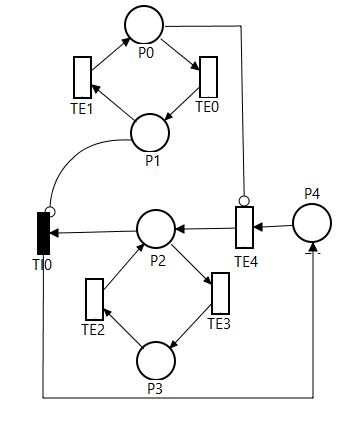
\includegraphics[scale=0.75]{img/cold-standby-example.png}}
\caption{Stochastic Petri net example}
\label{fig:stochastic_petri_net_example}
\end{figure}

Petri nets (PN) denote one great modeling mechanism used to describe simultaneous, asynchronous, shared, parallel, deterministic, and stochastic processes \citep{german2000performance}. These nets determine a term procedure that provides a numerical and graphical description and have scientific tools that allow for the confirmation of the features and exactness of illustrated systems. An extension of PNs is denoted as Stochastic Petri Nets (SPNs) \citep{marsan1998modelling}. SPNs mate a stochastic stop to an individually clocked transition. Hence, stochastic Petri nets can be isomorphic to continuous-time Markov chains (CTMC), and consequently they can give performance dimensions \citep{molloy1982integration}.

\subsection{Sensitivity analysis}

There are many methods for sensitivity analysis, among them we can mention the \textit{Differential Sensitivity Analysis (PD)}, \textit{Sensitivity Measures One at a Time}, \textit{The Relative Deviation Method (RD)}, \ textit{The Relative Deviation Rate (RDR)}, \textit{The partial rank correlation coefficient (PRCC)} and \textit{The Sensitivity Index (SI)} \citep{hamby1995comparison}. In our study, we will use the Sensitivity Index (SI), which uses the percentage difference technique for a simpler calculation.

The percentage difference technique for computing the sensitivity index $S_y(A)$, which indicates the impact on a given in availability caused by variations in an input parameter $y$. Equation 6 shows how the index of the sensitivity analysis is calculated for the y metric, where $max_y$ and $min_y$ represent the maximum and minimum output values, respectively, of the calculation varying the parameter y over the maximum value $max_y$ \citep{clemente2022availability}.

\begin{align}\label{eq:sa}
S_y(A) = \frac{max_y - min_y}{max_y}.
\end{align}

During calculation $S_y(A)$, the other parameters of the model need to be fixed. Thus, it is performed for all parameters to be calculated and to build the sensitivity analysis classification. This classification improves the predictability of increased availability.

\section{Proposed Methodology}\label{sec:methodology}

\begin{figure}[htbp]
\centerline{
\includegraphics[scale=0.6]{img/methodology.png}}
\caption{Methodology overview}
\label{fig:methodology}
\end{figure}

Figure \ref{fig:methodology} is a structure chart that summarizes our methodology in order. The rectangles represent each step of the methodology, and the arrows connected between the rectangles define the execution order. The diamond, on the other hand, represents a stage that can lead to two different paths, that is, if the results are considered satisfactory, the evaluation proceeds. Otherwise, it returns to one of the previous steps, and changes are made until it behaves close to what is expected of the real system.

The stage's \textit{Studying the system} and \textit{Building metrics of interest} were investigative stages where we carried out a careful analysis of the target system; seeking information from manufacturers, related work and observing the system's operation to then define metrics of interest that we could improve. These steps supported the following steps:

\textit{Building the models}, at this stage, after studying the system and defining the metrics of interest, we build two models with specific objectives; the first model represents the base system by continuous-time Markov chains, from which we extract the closed formula for variation of input parameters. The second model, made in Petri nets, represents the same base system with the addition of redundancy mechanisms applied to the UAV and power source.

\textit{Calculate the sensitivity rating and identify relevant components}, we used the Mercury tool \citep{maciel2017mercury} for the sensitivity analysis with the sensitivity index (IS) method; we did the analysis based on the model input parameters CTMC, generating a rank of the components that most impacted the metrics of interest.

\textit{Results and suggestions}, finally, through the rank generated in the previous step, we were able to identify the components that would need intervention, either in the form of improving the MTTF and MTTR or in the use of redundancy mechanisms that allow prolonging their failure. With this, we generate graphs simulating these improvements and redundancy mechanisms, varying the parameters used as input in the models and analyzing the impact on the metrics of interest. 

The models, assessments and raw data can be seen and understood by designers, analysts and administrators but hardly by senior management. Therefore, it is important to provide available graphical and textual interpretation to support the decision-making process\citep{melo2021distributed}. 

\section{Architecture and models}\label{sec:model}
%parei aqui
This section will present the system's base architecture (its basic operational mode). Two models are conceived to represent the availability of the systems. A continuous-time Markov chain analytical model and the numerical method conceived through stochastic Petri nets.

\begin{figure}[htbp]
\centerline{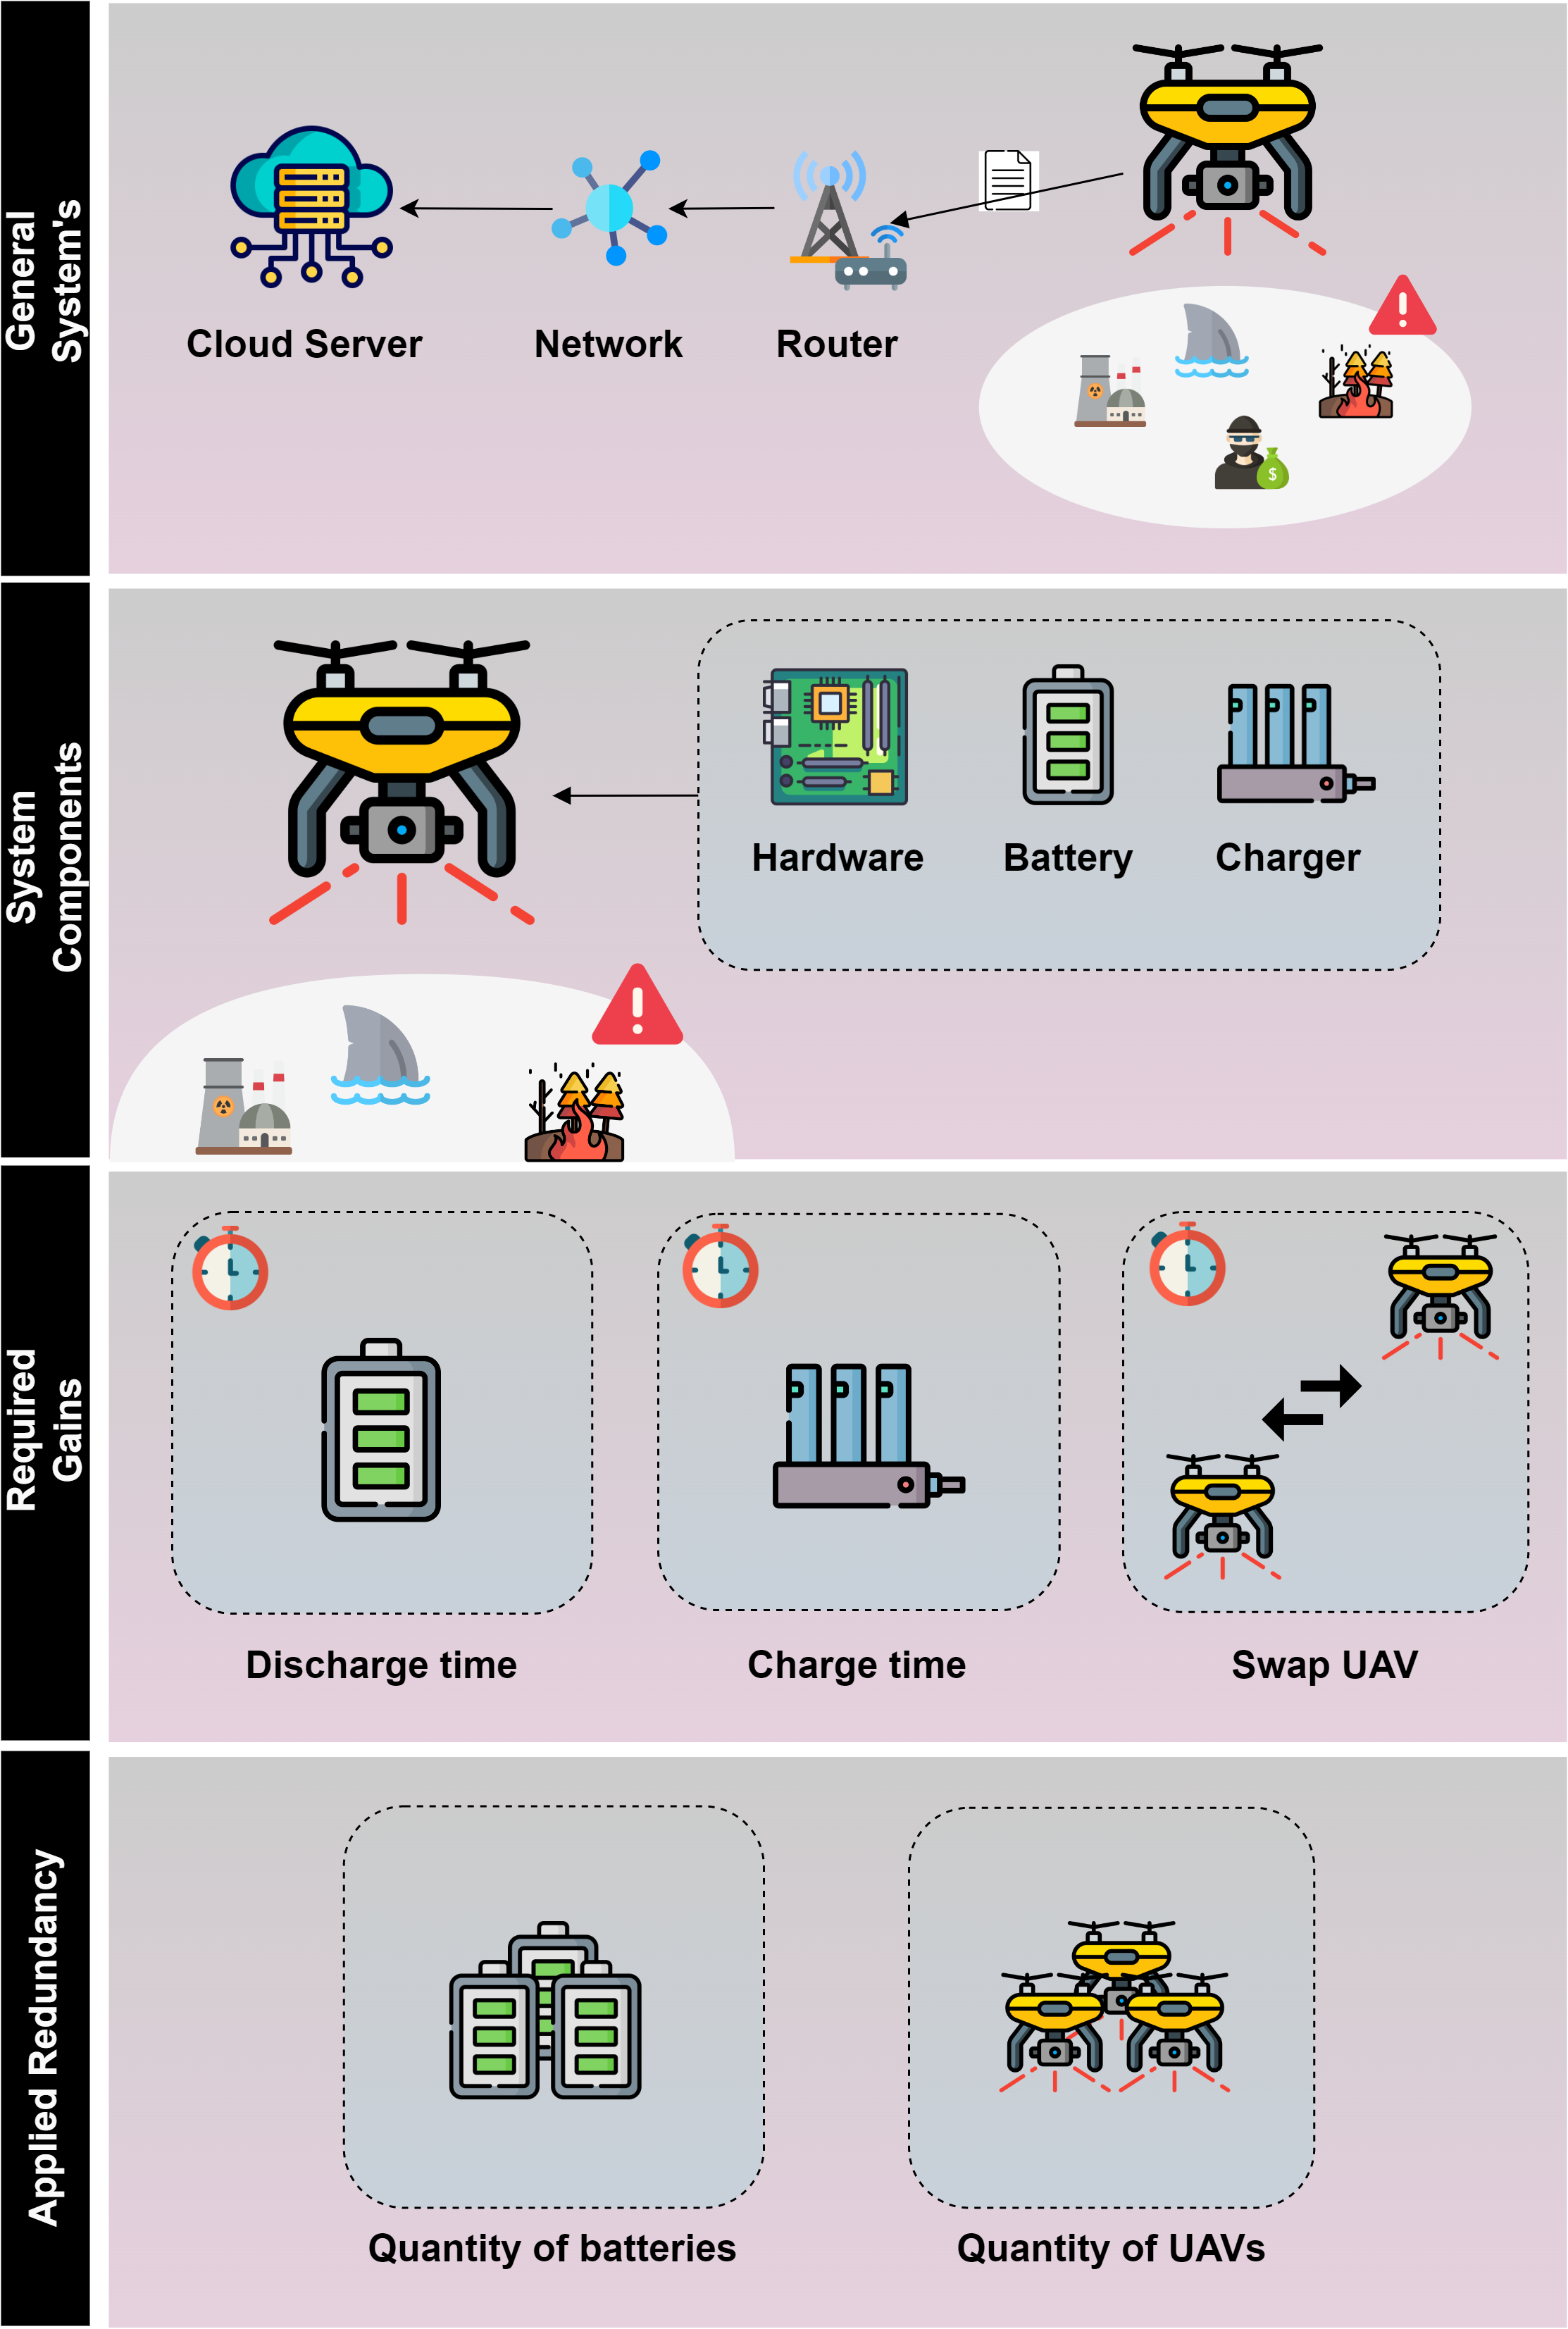
\includegraphics[scale=0.45]{img/operating_model.png}}
\caption{Overview of the Operating Mode}
\label{fig:operating_mode_overview}
\end{figure}

Figure \ref{fig:operating_mode_overview} depicts an overview of the evaluated system and the studies employed, broken down into \textit{General System}, \textit{System Components} of the UAV device, modes of \textit{Required Gains} to improve the system's availability, and \textit {Applied redundancy} that should be applied.

\textit{System}, we can observe the basic operating mode of the system; composed of a server, for data processing; a connection component, which in this case we are considering a router; and a UAV device for monitoring. The system is operational if, only if; the server, the router and the UAV is working. In the case of the UAV device, we are assuming that it is up and running if it is flying over the area of interest. 

\textit{Components}, shows the components of a UAV device that directly impact its availability, including the UAV device itself, its primary source of energy (battery) and its charging system.

\textit{Improvement}, in this partition, we have improvements in component times and UAV replacement (if considering redundancy methods) that can be applied to the base system in order to increase overall availability. It is important to note that the changeover time improvement is due to the development of an intelligent changeover system that will be able to trigger a reserve UAV before the active UAV returns to a landing base.  

\textit{Redundancy methods}, finally, we have the redundancy methods used that consider an increase in the number of spare batteries and UAVs to be replaced.


\begin{figure}[htbp]
\centerline{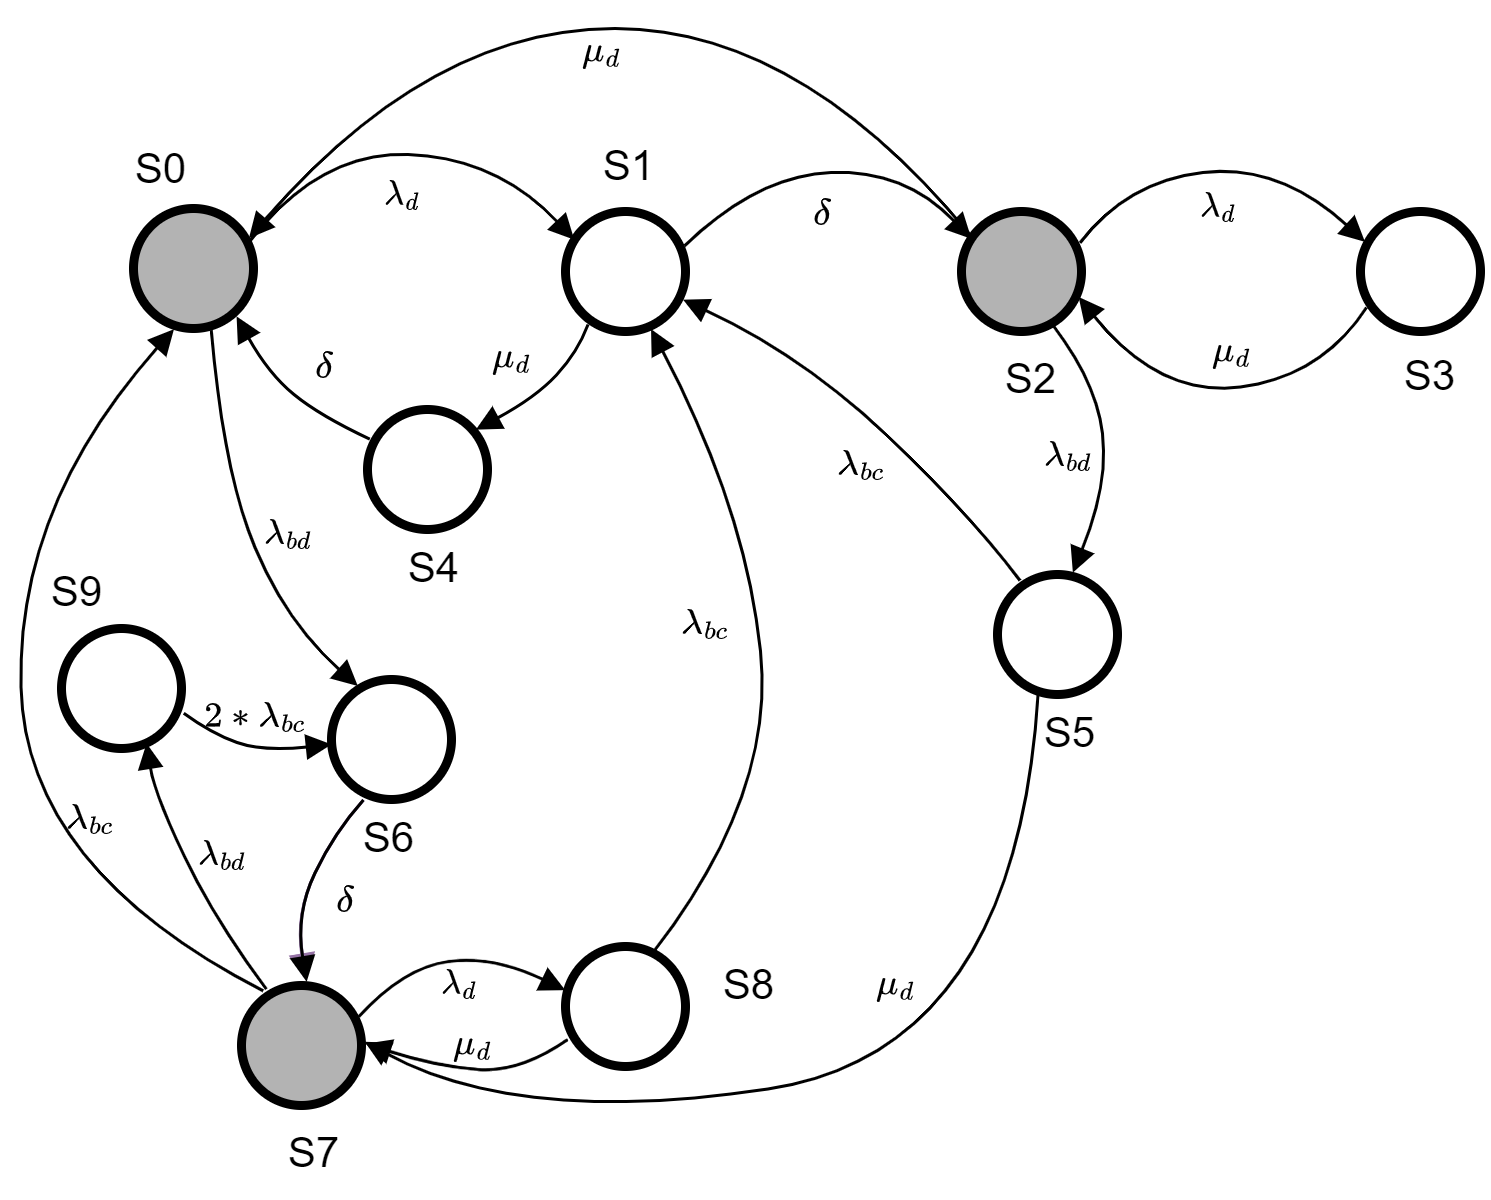
\includegraphics[scale=0.75]{img/CTMC_transparent.png}}
\caption{CTMC model of UAV flight system}
\label{fig:ctmc_model}
\end{figure}

\begin{table}[htbp]
\caption{Parameter Description for the CTMC model}
\begin{center}
\begin{tabular}{|c|c|}
\hline
\textbf{\textit{Parameter}}& \textbf{\textit{Description}} \\
\hline
  \(\lambda_{bd}\) & Battery discharge rate per hour \\
  \(\lambda_{bc}\)  & Battery charge rate per hour\\
 \(\mu_{d}\) & Drone repair rate per hour  \\
 \(\lambda_{d}\) & Drone failure rate per hour \\
 \(\delta\) & Drone swap rate per hour \\
\hline
\end{tabular}
\label{tab:ctmc_parameter_description}
\end{center}
\end{table}

In Figure \ref{fig:ctmc_model} we have our continuous-time Markov chain model representing the flight system of the UAV device, consisting of a drone in operation (flying drone), a drone and a power source as backup of replacement. The model evaluates the availability of the flight system, having as input parameters the charging rate ($\lambda_{bc}$) and discharging ($\lambda_{bd}$) of the drone battery per hour, as well as the rate device hardware failure ($\mu_{d}$) and repair ($\lambda_{d}$) per hour. The exchange rate between the operating drone and a backup drone per hour is also considered in $\delta$, this exchange rate includes landing time, battery replacement and takeoff for return (Table \ref{tab:ctmc_parameter_description}).

In circle formula we have the possible states to be reached by the system, states illustrated in dark color as the set of states $\{S0, S2, S7\}$ represent the operating system, that is, at least one drone is flying over the area of interest or processing the information. Therefore, the other states represent the system offline, with some drones broken or unloaded and no drones or power sources to replace.

From this Markov chain model, we were able to extract the analytical model, which will serve as a basis for architects and designers in the construction of a system with these characteristics. It is important to note that we are considering exponentially distributed times, which made it possible to extract the closed formula illustrated by the equation \ref{eq:a_uav}.

\begin{align}\label{eq:a_uav}
A_{UAV} = \frac{\delta  \lambda_{bc} \mu_{d} (\alpha_{2} \delta \phi_{2} + \beta_{2} \mu_{d} \phi_{1})}{ \alpha_{2} \delta^{2} \theta_{2} + \lambda_{bc} \mu_{d} (\alpha_{3} \delta  \lambda_{bc} \lambda_{bd} \lambda_{d} + \theta_{1} \mu_{d})+ \beta_{2} \mu_{d}^{3} \phi_{3}}
\end{align}

Where: \\

\begin{minipage}{.8\textwidth}%  
\(\beta = \lambda_{bd} + \lambda_{d};\) \\
\(\beta_{2} = \lambda_{bd} + \mu_{d};\) \\
\(\beta_{3} = \lambda_{d} + \mu_{d};\) \\
\(\beta_{4} = \lambda_{bc} + \lambda_{bd};\) \\
\(\beta_{5} = \lambda_{bc} + \mu_{d};\) \\
\(\alpha_{1} = \beta + \lambda_{bc};\) \\
\(\alpha_{2} = \beta + \beta_{5};\) \\
\(\alpha_{3} = \beta_{3} + \beta_{4};\) \\
\(\alpha_{4} = \beta_{3}\lambda_{bc} + \lambda_{bd} \mu_{d};\) \\
\(\phi_{1} = \alpha_{1}\lambda_{bc} + \beta_{4} \mu_{d};\) \\
\(\phi_{2} = \beta_{3}\lambda_{bc} + \lambda_{bd} \mu_{d};\) \\
\(\phi_{3} = \beta \lambda_{bc}^{2} + \lambda_{bd} (\lambda_{bd} (\delta + \lambda_{bc}) + 2 \delta \lambda_{bc});\) \\
\(\phi_{4} = \beta_{3}^{2} + \beta_{3} (\lambda_{bc} + 3 \lambda_{bd}) + \lambda_{bd} (2 \lambda_{bc} + 3 \lambda_{bd});\) \\
\(\phi_{5} = \lambda_{d}^{2} + \lambda_{d} \mu_{d} + \mu_{d}^{2} ;\) \\
\(\theta_{1} = \alpha_{1} \beta  \beta_{2} \lambda_{bc} + 2 \beta  \beta_{2}  \delta \lambda_{bd}+ \delta  \lambda_{bc} \phi_{4};\) \\
\(\theta_{2} =  \alpha_{4} \lambda_{bd} \mu_{d} + \lambda_{bc}^{2} \phi_{5};\) \\
\end{minipage}%

We also include the formula for availability of other components necessary for the functioning of a monitoring system like this, composed of a server and a connection device exemplified here as a router, its analytical formulas are shown in the equations \ref{eq:a_server} and \ref{eq:a_router}, respectively. However, we do not consider them in our sensitivity analyzes and in the assessment of system availability. Components such as the server and the router have high availability compared to the UAV device, considered by us as the major bottleneck of the overall system and selected for an availability improvement analysis.

\begin{align}\label{eq:a_server}
A_{Server} = \frac{\lambda_{hw}}{\lambda_{hw} + \mu_{hw}} \times \frac{\lambda_{os}}{\lambda_{os} + \mu_{os}} \times
\frac{\lambda_{hp}}{\lambda_{hp} + \mu_{hp}} 
\end{align}

\[\times(1- (\frac{\mu_{vm}}{\lambda_{vm} + \mu_{vm}})^{3})\]

\begin{align}\label{eq:a_router}
A_{R} = \frac{\lambda}{\lambda + \mu} 
\end{align}

The analytical model of server availability (Equation \ref{eq:a_server}) and router (Equation \ref{eq:a_router}) has in its structure the failure rate, represented by $\lambda$ and the repair rate $\mu $. However, the server availability model is composed of the product of the hardware availability models ($hw$), operating system ($os$), virtual machine management hypervisor ($hp$), and virtual machine model ($ vm$); components commonly used for processing a monitoring system.

\begin{align}\label{eq:a}
A = A_{Server} \times A_{R}  \times A_{UAV}
\end{align}

The general availability of the system is given by Equation \ref{eq:a}, where we have the product of the server, router and UAV flight system availability models.

The UAV flight system availability analytical model (Equation \ref{eq:a_uav}) extracted from CTMC considers only the system in basic operating mode, ie; 1 in-flight UAV, 1 backup UAV, 1 backup battery. As already seen, we can use it to vary the failure and repair times of the UAV, battery and recharging components to improve the availability metric. However, in order to include redundancy mechanisms in this model and have a system with a more advanced operating mode, we would have a model with a giant and unfeasible state space for calculating availability.

In view of the problem of giant state space in Markov chains and analytical models extracted from it impossible to be calculated by a person, we then propose an approach with a numerical method model of stochastic Petri nets (SPN) that can be evaluated using computational tools such as Mercury \cite{maciel2017mercury}.

\begin{figure}[htbp]
\centerline{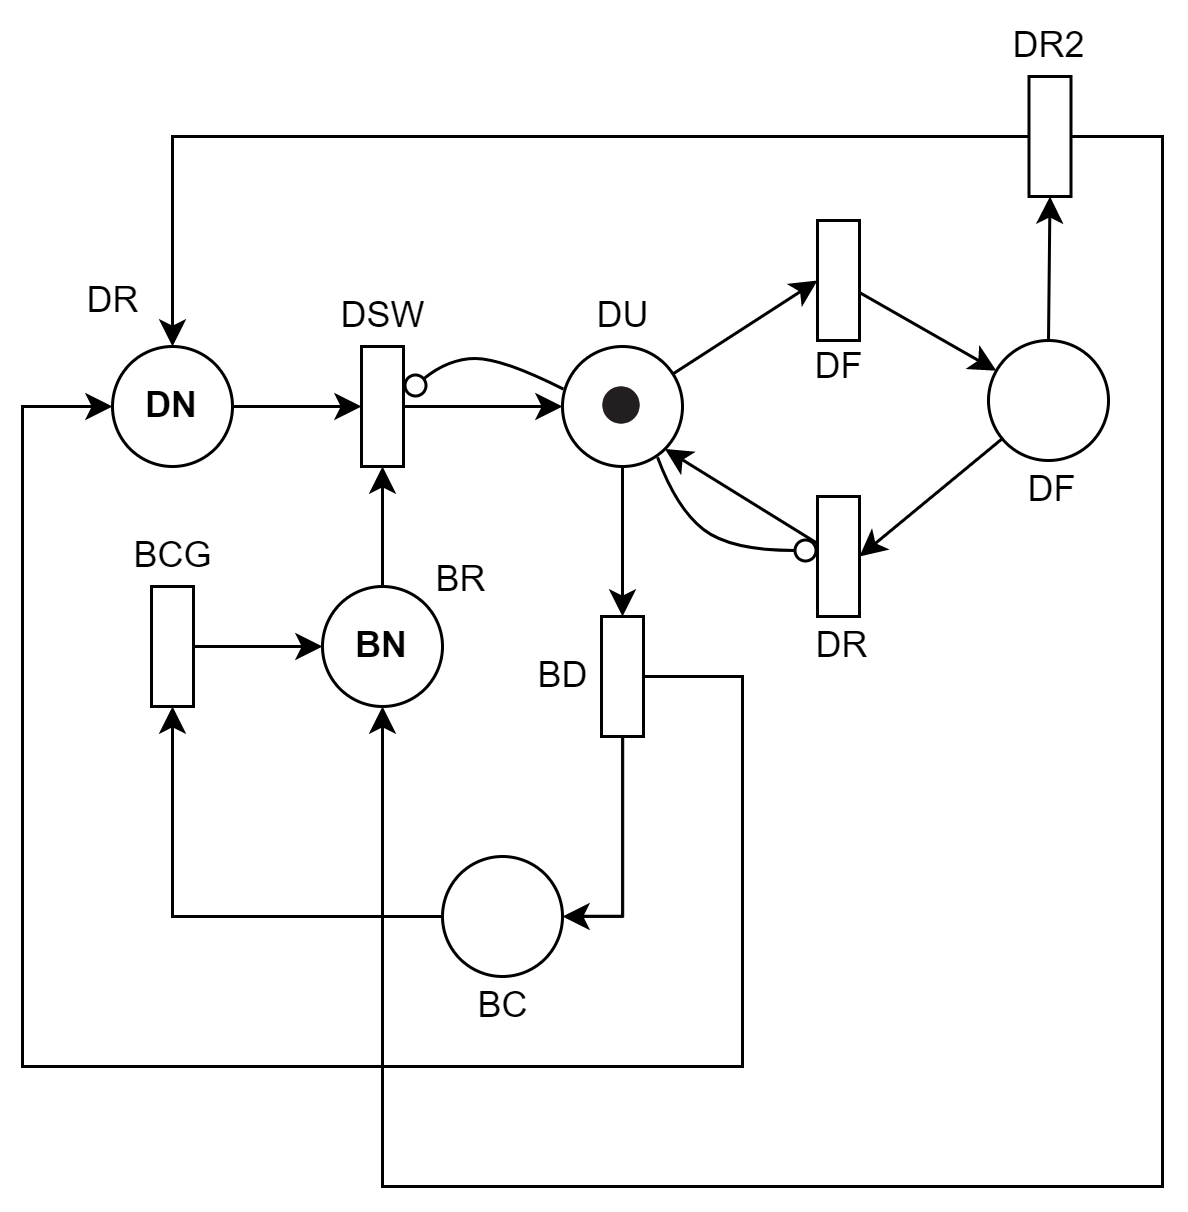
\includegraphics[scale=0.7]{img/SPN_transparent.png}}
\caption{SPN model of UAV flight system}
\label{fig:spn_model}
\end{figure}

\begin{table}[htbp]
\caption{Parameter Description for the SPN model}
\begin{center}
\begin{tabular}{|c|c|c|}
\hline
\textbf{\textit{Transition}} & \textbf{\textit{Parameter}}& \textbf{\textit{Description}} \\
\hline
 DF & MTTFD & Mean time to drone failure \\
 DR & MTTRD & Mean time to drone repair\\
 DR2 & MTTRD & With guard \textbf{$\#DU>0$} \\
 BD & MTTBD & Mean time to battery discharge \\ 
 BCG & MTTBC & Mean time to battery charge \\
 DSW & MTTSD & Mean time to swap drone \\
\hline
\end{tabular}
\label{tab:spn_parameter_description}
\end{center}
\end{table}

The SPN model represented by Figure \ref{fig:spn_model} was used to model the use of redundancy mechanisms in the system, its architecture is converted back to a CTMC state space, but fully processed by the machine.

The place (circle) \textbf{DU} marks the system as working, while the place \textbf{DF} indicates a failed state. The other places: \textbf{DR}, \textbf{BR} and \textbf{BC}; indicate the amount of spare UAVs, spare batteries and charging batteries respectively.

Initially 1 UAV is operational, with 1 UAV and battery backup. The UAV has a mean time to failure (MTTF) and a mean time to repair (MTTR), as well as an average loading, unloading and swapping time. These times follow an exponential distribution, represented in the model by timed transitions (white rectangles) connected by arcs to the state places. All mean time parameters (MTT's) used as input to the model can be seen in Table \ref{tab:spn_parameter_description} per transition belonging.

There are two types of arcs in the proposed model, the arc that ends with an arrow is the most common, and indicates the activation of a transition if the requirements are met, and the movement of a token (the small black circle inside a place, which indicates the number of features), while the arc that ends with a circle is called an inhibitor arc. An inhibitor arc indicates that a transition can only be activated if certain conditions are met. Timed transitions depend on the time to activate and the black rectangle is the transition called immediate transition, which can be activated if the required amount of tokens is present in the connected location \citep{melo2021distributed}.

\section{Case studies}\label{sec:case_studies}
The purpose of this section is to present two case studies showing the use of the suggested technique to evaluate scenarios in an unmanned aerial vehicle (UAV) flight system. They are based on an analysis of availability and downtime measurements.

To start the evaluation with the models we need to define the system parameter values in the basic operating mode (see section \ref{sec:model}).. These values were collected from manufacturers' websites.

\textit{Case Study 1} 

uses offered sensitivity analysis methodologies to identify parameters in drone flight system availability that require improvement.

\textit{case study 2} 

assesses whether the sensitivity analysis performed in case study 1 significantly increases system availability and then provides alternative redundancy mechanisms to achieve greater availability in the system's basic operating mode.

Finally, \textit{case study 3} uses the improvements of case study 1 in MTT parameters to apply redundancy mechanisms on top of these improvements. The combination of the two methods used in case study 1 and 2 can be considered when planning to evaluate a compromise between cost and availability. Designers and architects can choose to improve system components or increase their redundancy based on cost.

In order to guide ourselves on which rate or MTT of the system we could vary its values first to obtain a better availability metric, we calculate a sensitivity rank through the percentage differentiation technique defined by the equation \ref{eq:sa}, where the order of the parameter of the component that has the greatest impact on system availability (TABLE \ref{tab:sa_rank}).

\begin{table}[htbp]
\caption{Sensitivity ranking obtained through}
\begin{center}
\begin{tabular}{|c|c|c|}
\hline
\textbf{\textit{Parameter}}& \textbf{\textit{Ranking}} & \textbf{\textit{Sensitivity index}} \\
\hline
\(\lambda_{bd}\) & 1st & -3.720460029055 \\
\(\lambda_{bc}\) & 2nd & 3.3226751100809997 \\
 \(\mu_{d}\) & 3rd & -1.064622392094 \\
\(\lambda_{d}\) & 4th & 0.9995887722079999 \\
\(\delta\) & 5th & 0.462793032533 \\
\hline
\end{tabular}
\label{tab:sa_rank}
\end{center}
\end{table}

In the sensitivity analysis performed, we have the discharging rate per hour connected to the battery component as the parameter that most impacts the availability of the system according to the sensitivity index in column 3 of the table, followed by the charging rate per hour, repair rate, failure rate and UAV exchange rate.

\subsection{Case study 1}\label{sec:case_studies_sub01}

\begin{figure}[htbp]
\centerline{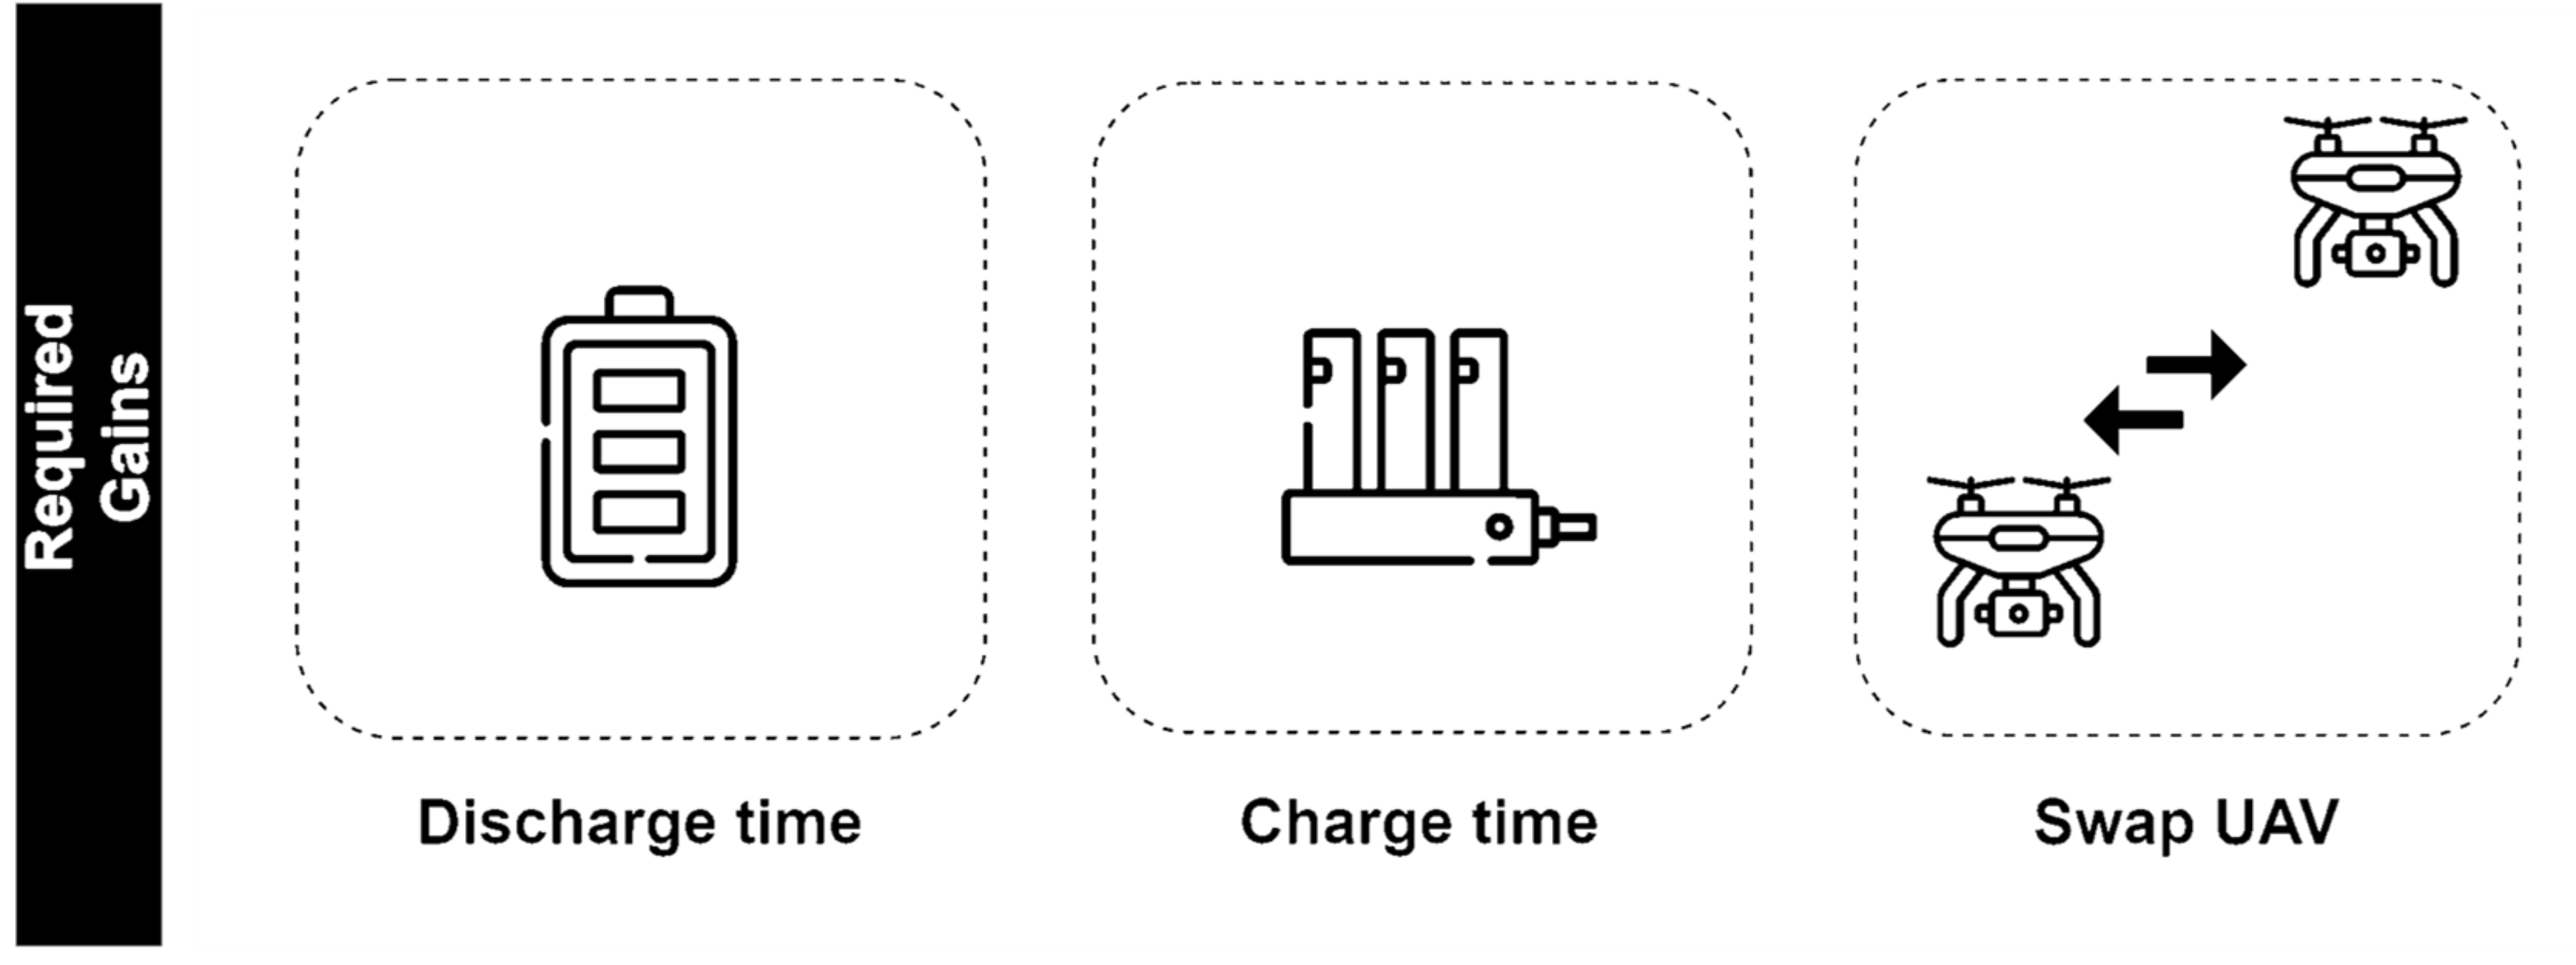
\includegraphics[scale=0.2]{img/operating_model_study_01.png}}
\caption{Required Gains}
\label{fig:case_study_01}
\end{figure}

\begin{figure}[htbp]
\centerline{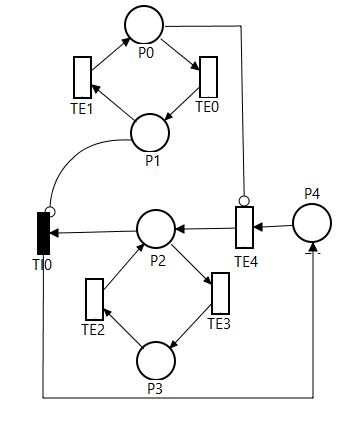
\includegraphics[scale=0.75]{img/cold-standby-example.png}}
\caption{Stochastic Petri net example}
\label{fig:stochastic_petri_net_example}
\end{figure}

In this case study we use the analytical model and also the CTMC flight system availability of UAV devices to increase availability by improving the input parameters. System baseline parameter values are shown in table \ref{tab:spn_parameter_values} and variation graphs in Figure \ref{fig:ctmc_sa}.

\begin{table}[htbp]
\caption{Parameter values for the CTMC model}
\begin{center}
\begin{tabular}{|c|c|}
\hline
\textbf{\textit{Parameter}} & \textbf{\textit{Value (rate)}} \\
\hline
  \(\lambda_{bd}\)  & 2 \\
  \(\lambda_{bc}\)   & 0.5 \\
 \(\mu_{d}\)   & 0.5  \\
 \(\lambda_{d}\)  & 0.0002 \\
 \(\delta\)  & 6 \\
\hline
\end{tabular}
\label{tab:ctmc_parameter_values}
\end{center}
\end{table}

Parameter values are given in rate format (amount per hour) for input to Markov chain and analytical models (section \ref{sec:background}). Where, $\lambda_{bd}$ is 2 (two) discharges per hour, $\lambda_{bc}$ is 0.5 (half) charge per hour, $\mu_{d}$ 0.5 (half) repair per hour, $ \lambda_{d}$ is 0.0002 failures per hour and $\delta$ is 6 UAV changes per hour.

Initially, we started our analysis by varying the value of $\lambda_{bd}$ (battery discharge rate), set this at an improved value, and varied the next one, the $\lambda_{bc}$ (charging rate). Finally, we vary the swap parameter ($\delta$) with $\lambda_{bd}$ and $\lambda_{bc}$ set to their improved values. The UAV repair fee ($\mu_{d}$) and failure fee ($\lambda_{d}$) values have not changed; their baseline values had little impact on overall availability.

\begin{figure}[htbp]
     \centering
     \begin{subfigure}[b]{0.45\textwidth}
         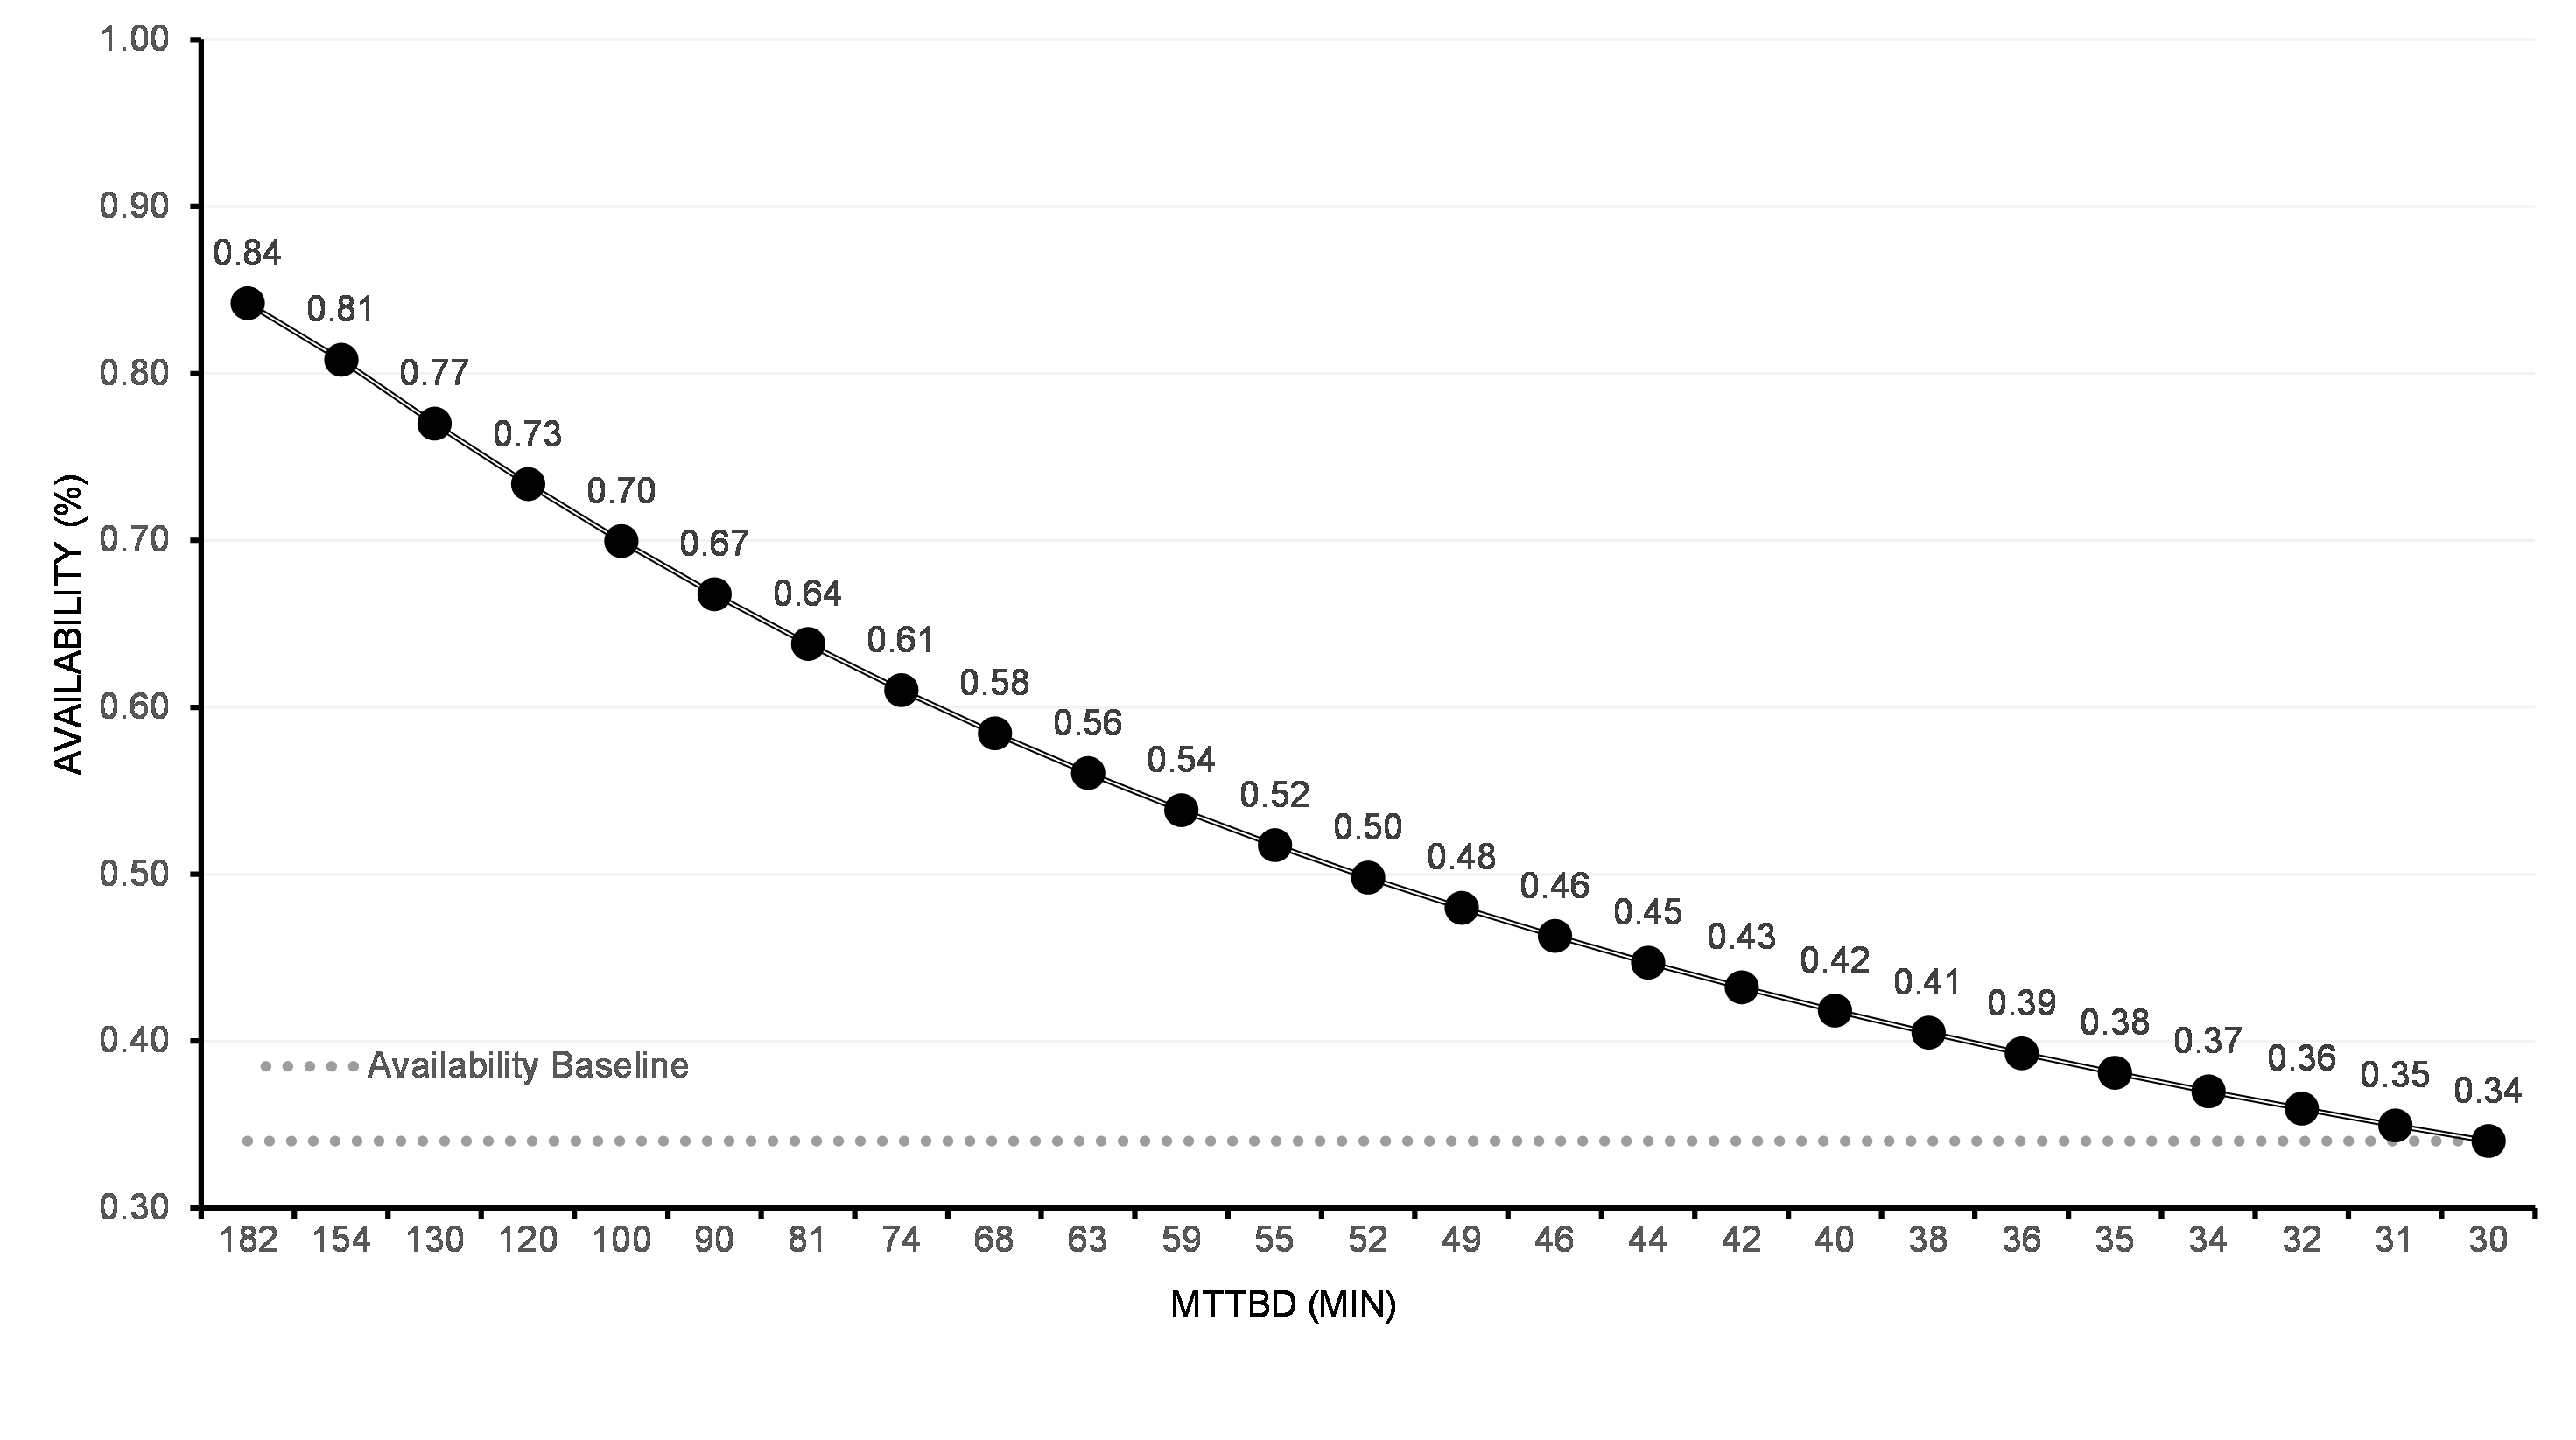
\includegraphics[width=\linewidth]{img/exps/SA_007.png}
         \caption{}
         \label{fig:ctmc_sa_bd}
     \end{subfigure}
     \hfill
     \begin{subfigure}[b]{0.45\textwidth}
         \centering
         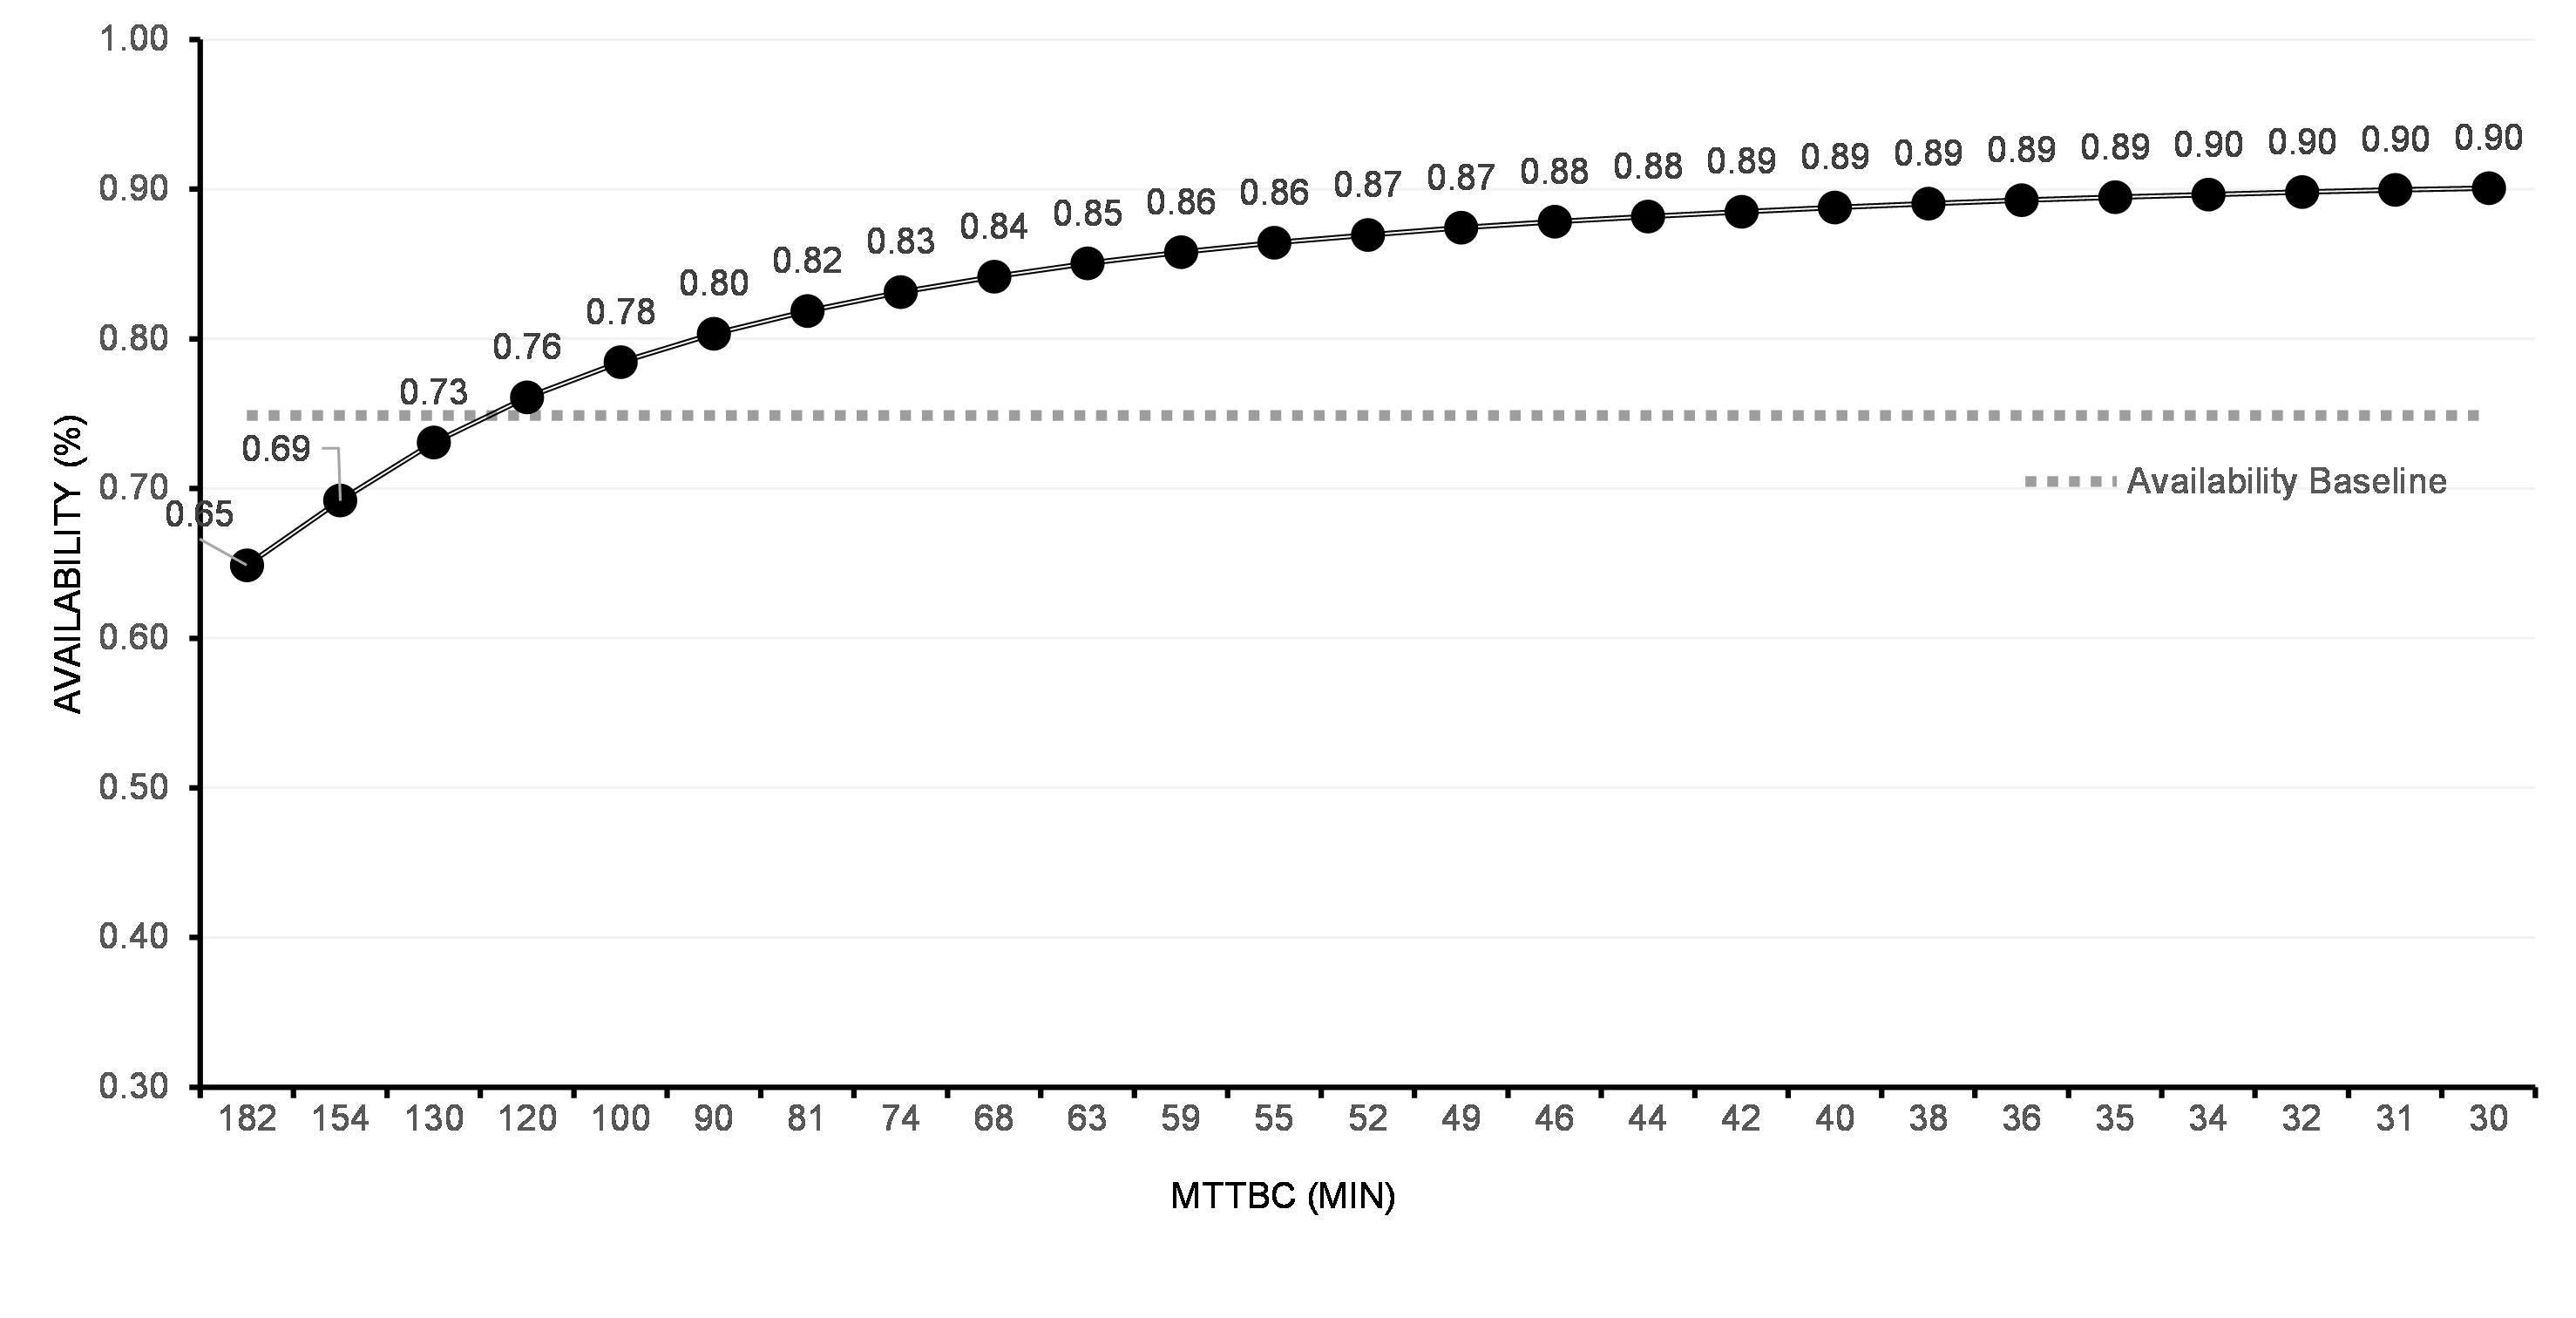
\includegraphics[width=\linewidth]{img/exps/SA_001.png}
         \caption{}
         \label{fig:ctmc_sa_bc}
     \end{subfigure}
     \hfill
     \begin{subfigure}[b]{0.45\textwidth}
         \centering
         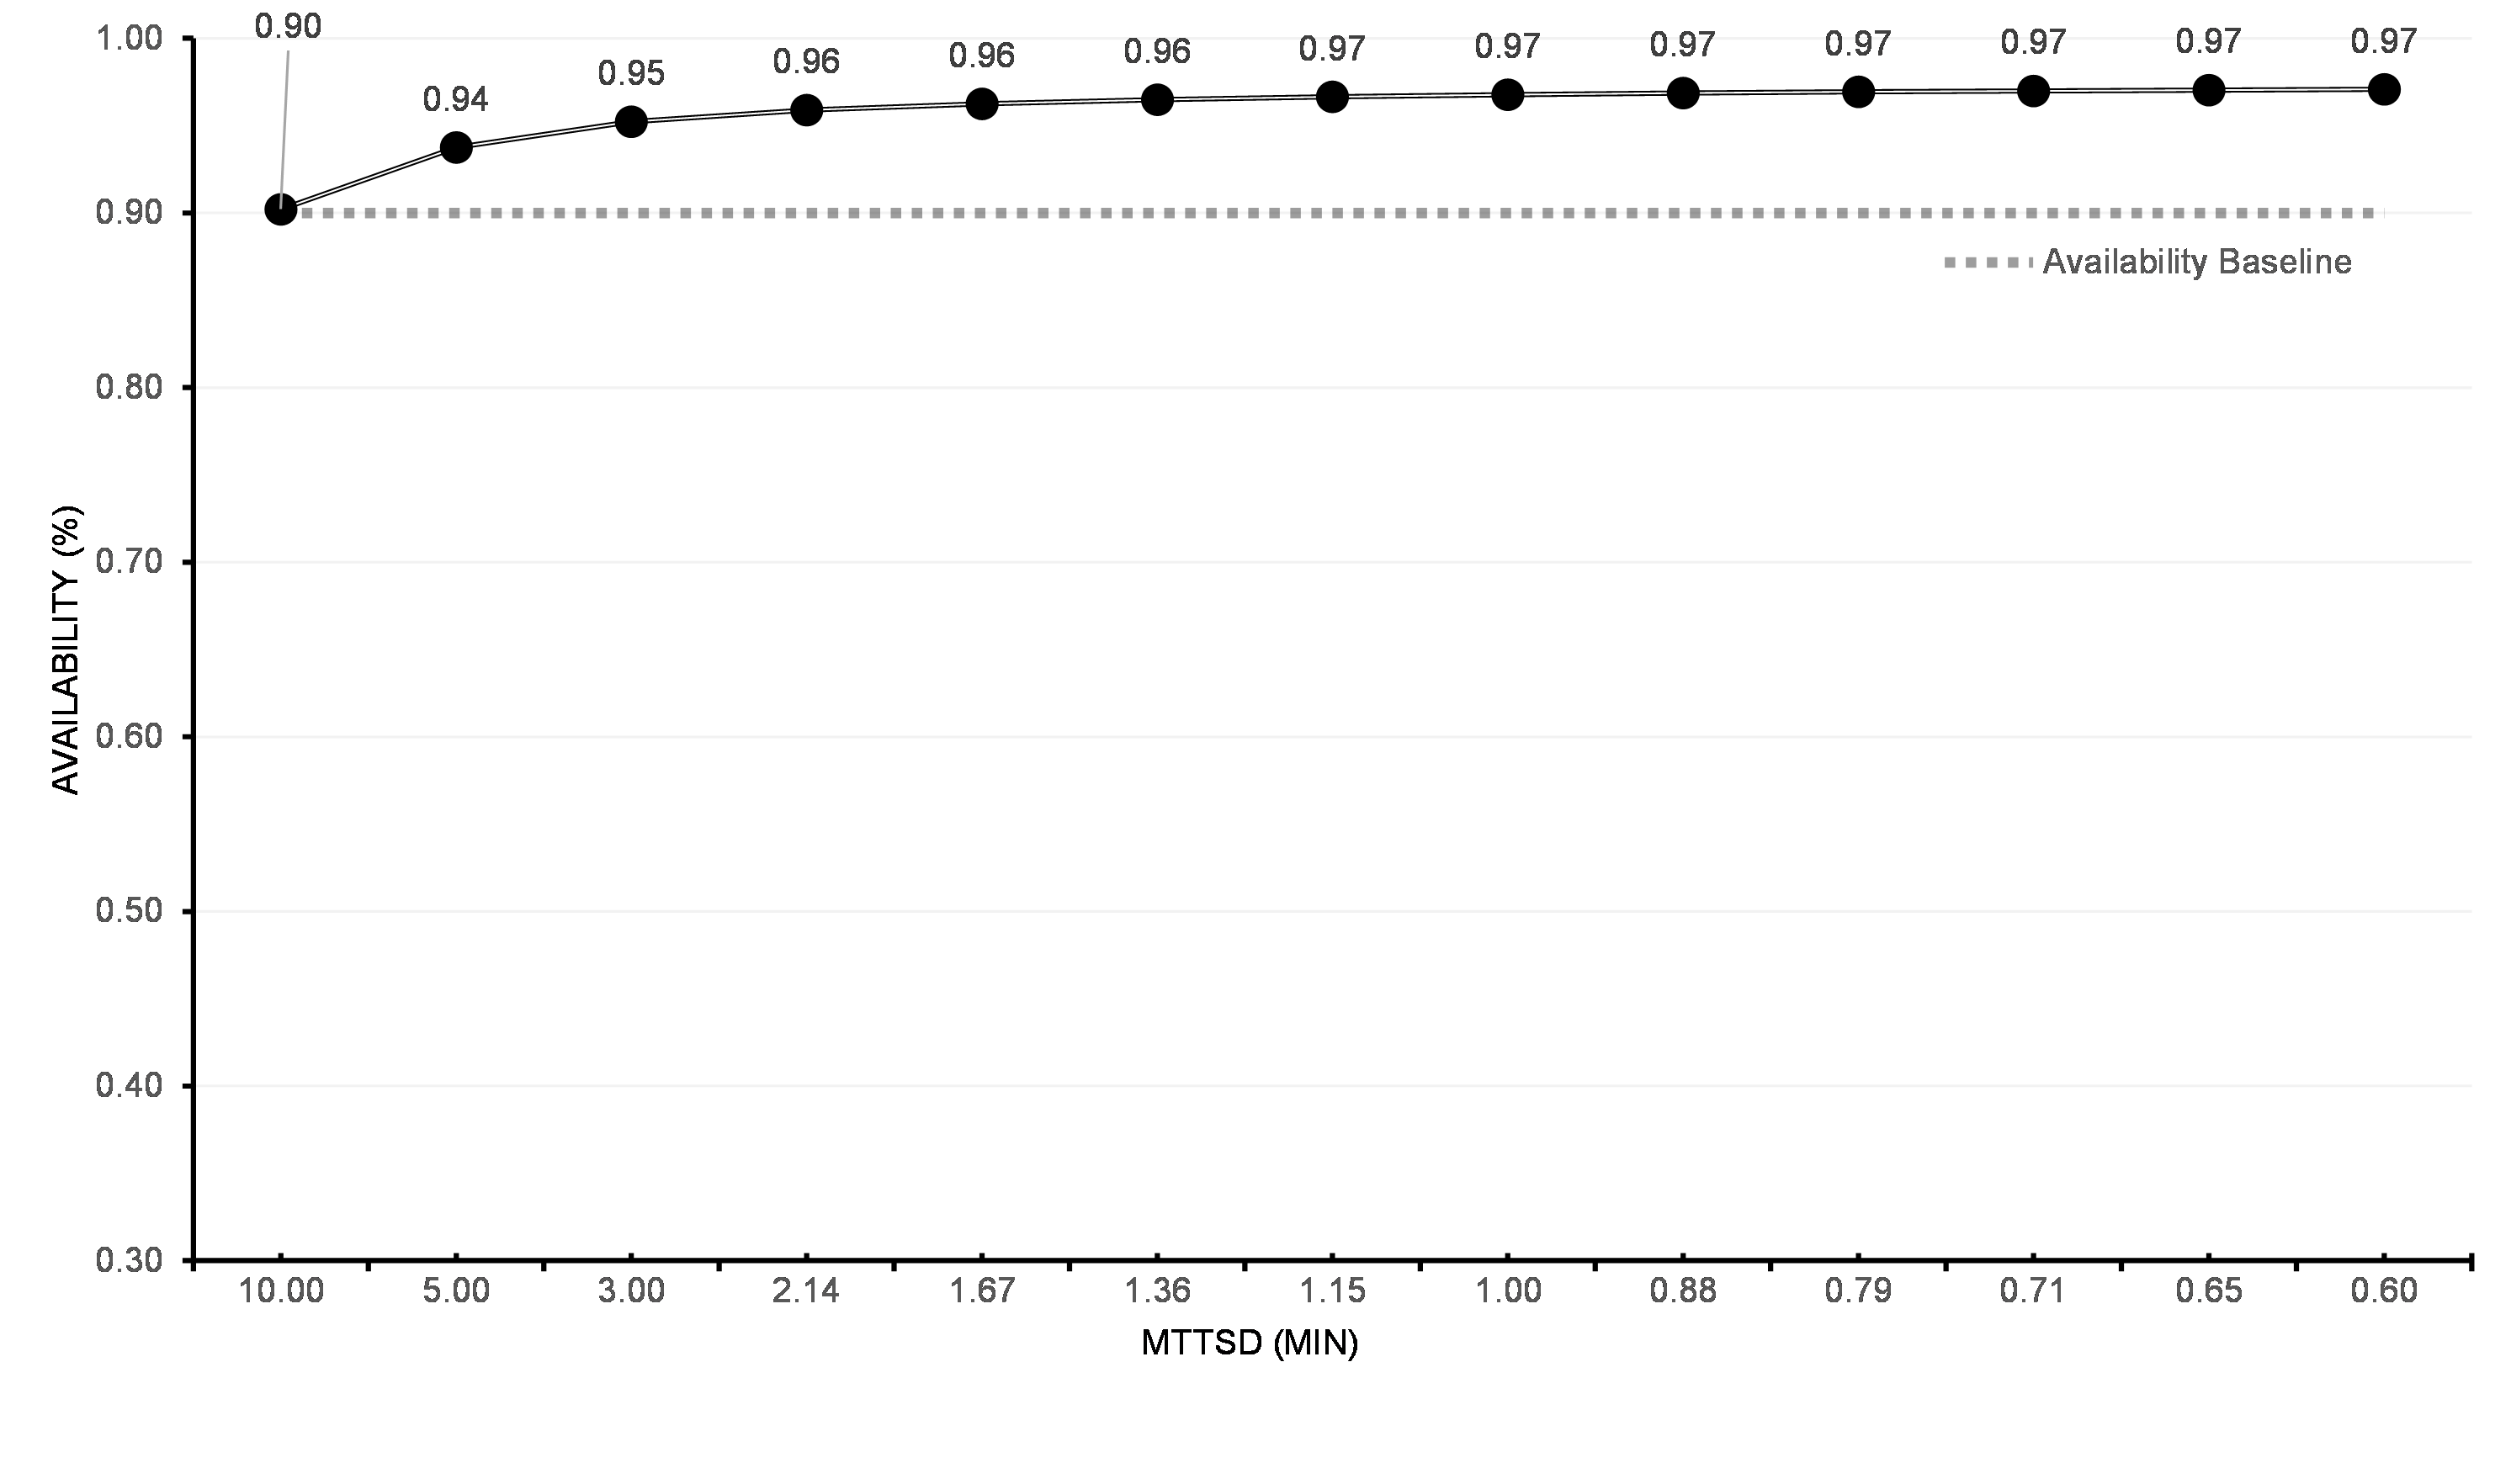
\includegraphics[width=\linewidth]{img/exps/SA_002.png}
         \caption{}
         \label{fig:ctmc_sa_suav}
     \end{subfigure}
        \caption{Variation one by one}
        \label{fig:ctmc_sa}
\end{figure}

In Figure \ref{fig:ctmc_sa_bd} we have the graph of variation of $\lambda_{bd}$ and we can see the availability of the baseline system represented by $\lambda_{bd}$ equal to 2 discharges per hour or 30 minutes of flight as it is on the chart (in minutes). By improving the flight time of the UAV device, we can go from an availability of 0.34\% of the time to 0.84\% with 180 minutes of flight (3 hours). 

Going to the variation graph (Fig. \ref{fig:ctmc_sa_bc}) (charging time), we have an availability improvement of about nine (0.90\%) with 30 minutes of charging and a flight time fixed at 90 minutes. Finally, we achieved an availability of 0.97\% in a UAV exchange of less than 1.30 minutes (Fig. \ref{fig:ctmc_sa_suav}).



\subsection{Case study 2}\label{sec:case_studies_sub02}

\begin{figure}[htbp]
\centerline{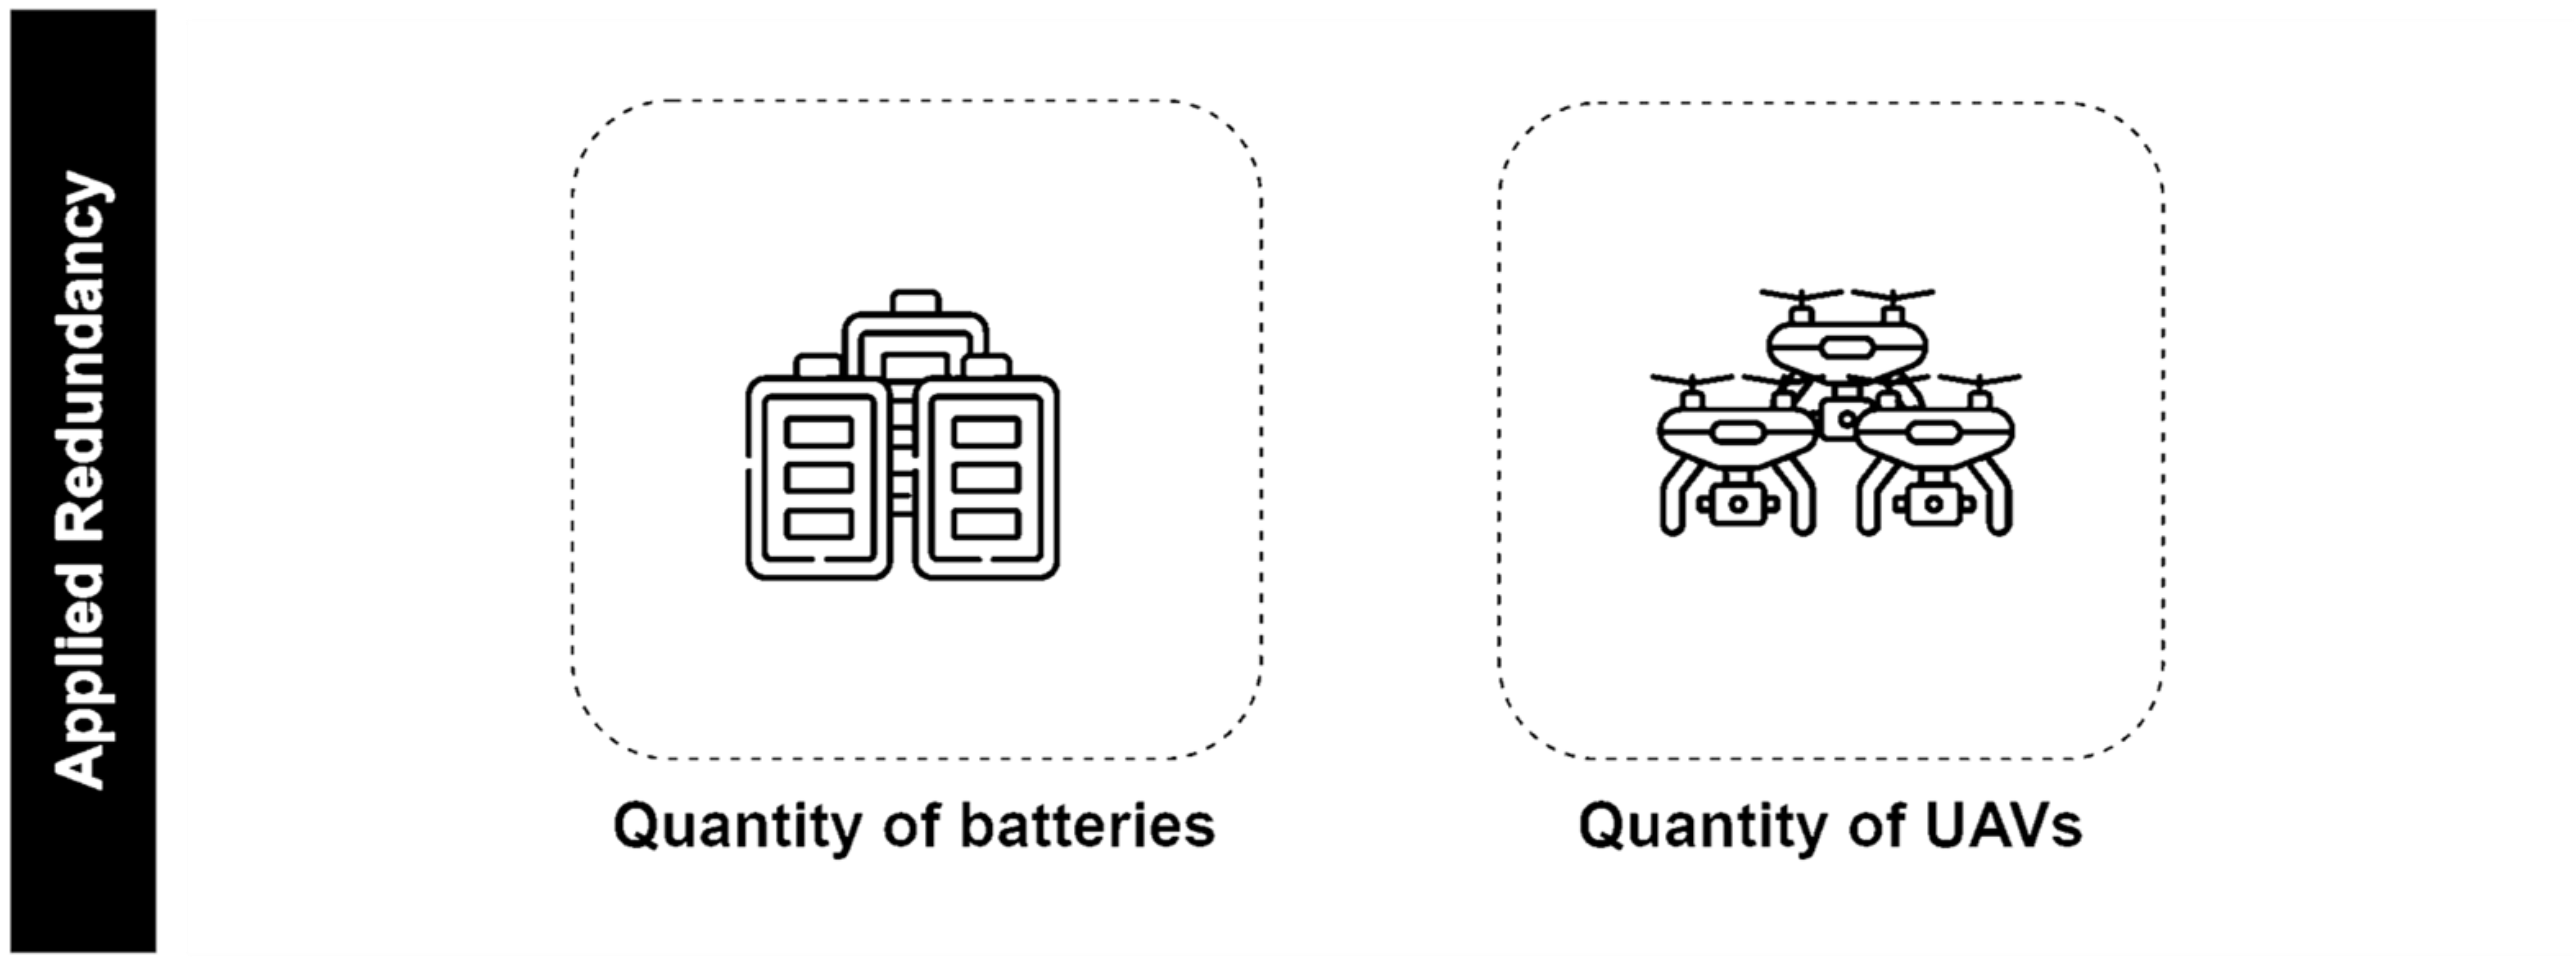
\includegraphics[scale=0.22]{img/operating_model_study_02.png}}
\caption{Applied Redundancy}
\label{fig:case_study_02}
\end{figure}

To generate models with redundancy techniques using continuous-time Markov chains (CTMC) or even analytical models with equations, we would have to face the explosion of states, which makes it difficult to understand the CTMC and manually calculate the generated analytical equations.

In this case study, we will use a new availability model for the flight system of UAVs; a model of stochastic Petri nets (SPN), which facilitates the modeling of systems with redundancy mechanisms. SPNs are numerical models evaluated by simulation via software. For this study, we will use the Mercury tool to evaluate the \citep{maciel2017mercury} model.

The values of input parameters of the SPNs are given by times (MTTs). In the table \ref{tab:basic_spn_parameter_values} we have the MTTs of the baseline system composed of the same values of case study 1 in time format.


\begin{table}[htbp]
\caption{Parameter values for the SPN model}
\begin{center}
\begin{tabular}{|c|c|}
\hline
\textbf{\textit{Parameter}} & \textbf{\textit{Value (hours)}} \\
\hline
  MTTFD & 5000\\
 MTTRD & 2\\
 MTTBD & 0.5 \\ 
 MTTBC & 2 \\
 MTTSD & 0.166666667 \\
 NB & 1 \\
 ND & 1 \\
\hline
\end{tabular}
\label{tab:basic_spn_parameter_values}
\end{center}
\end{table}

\begin{figure}[htbp]
\centerline{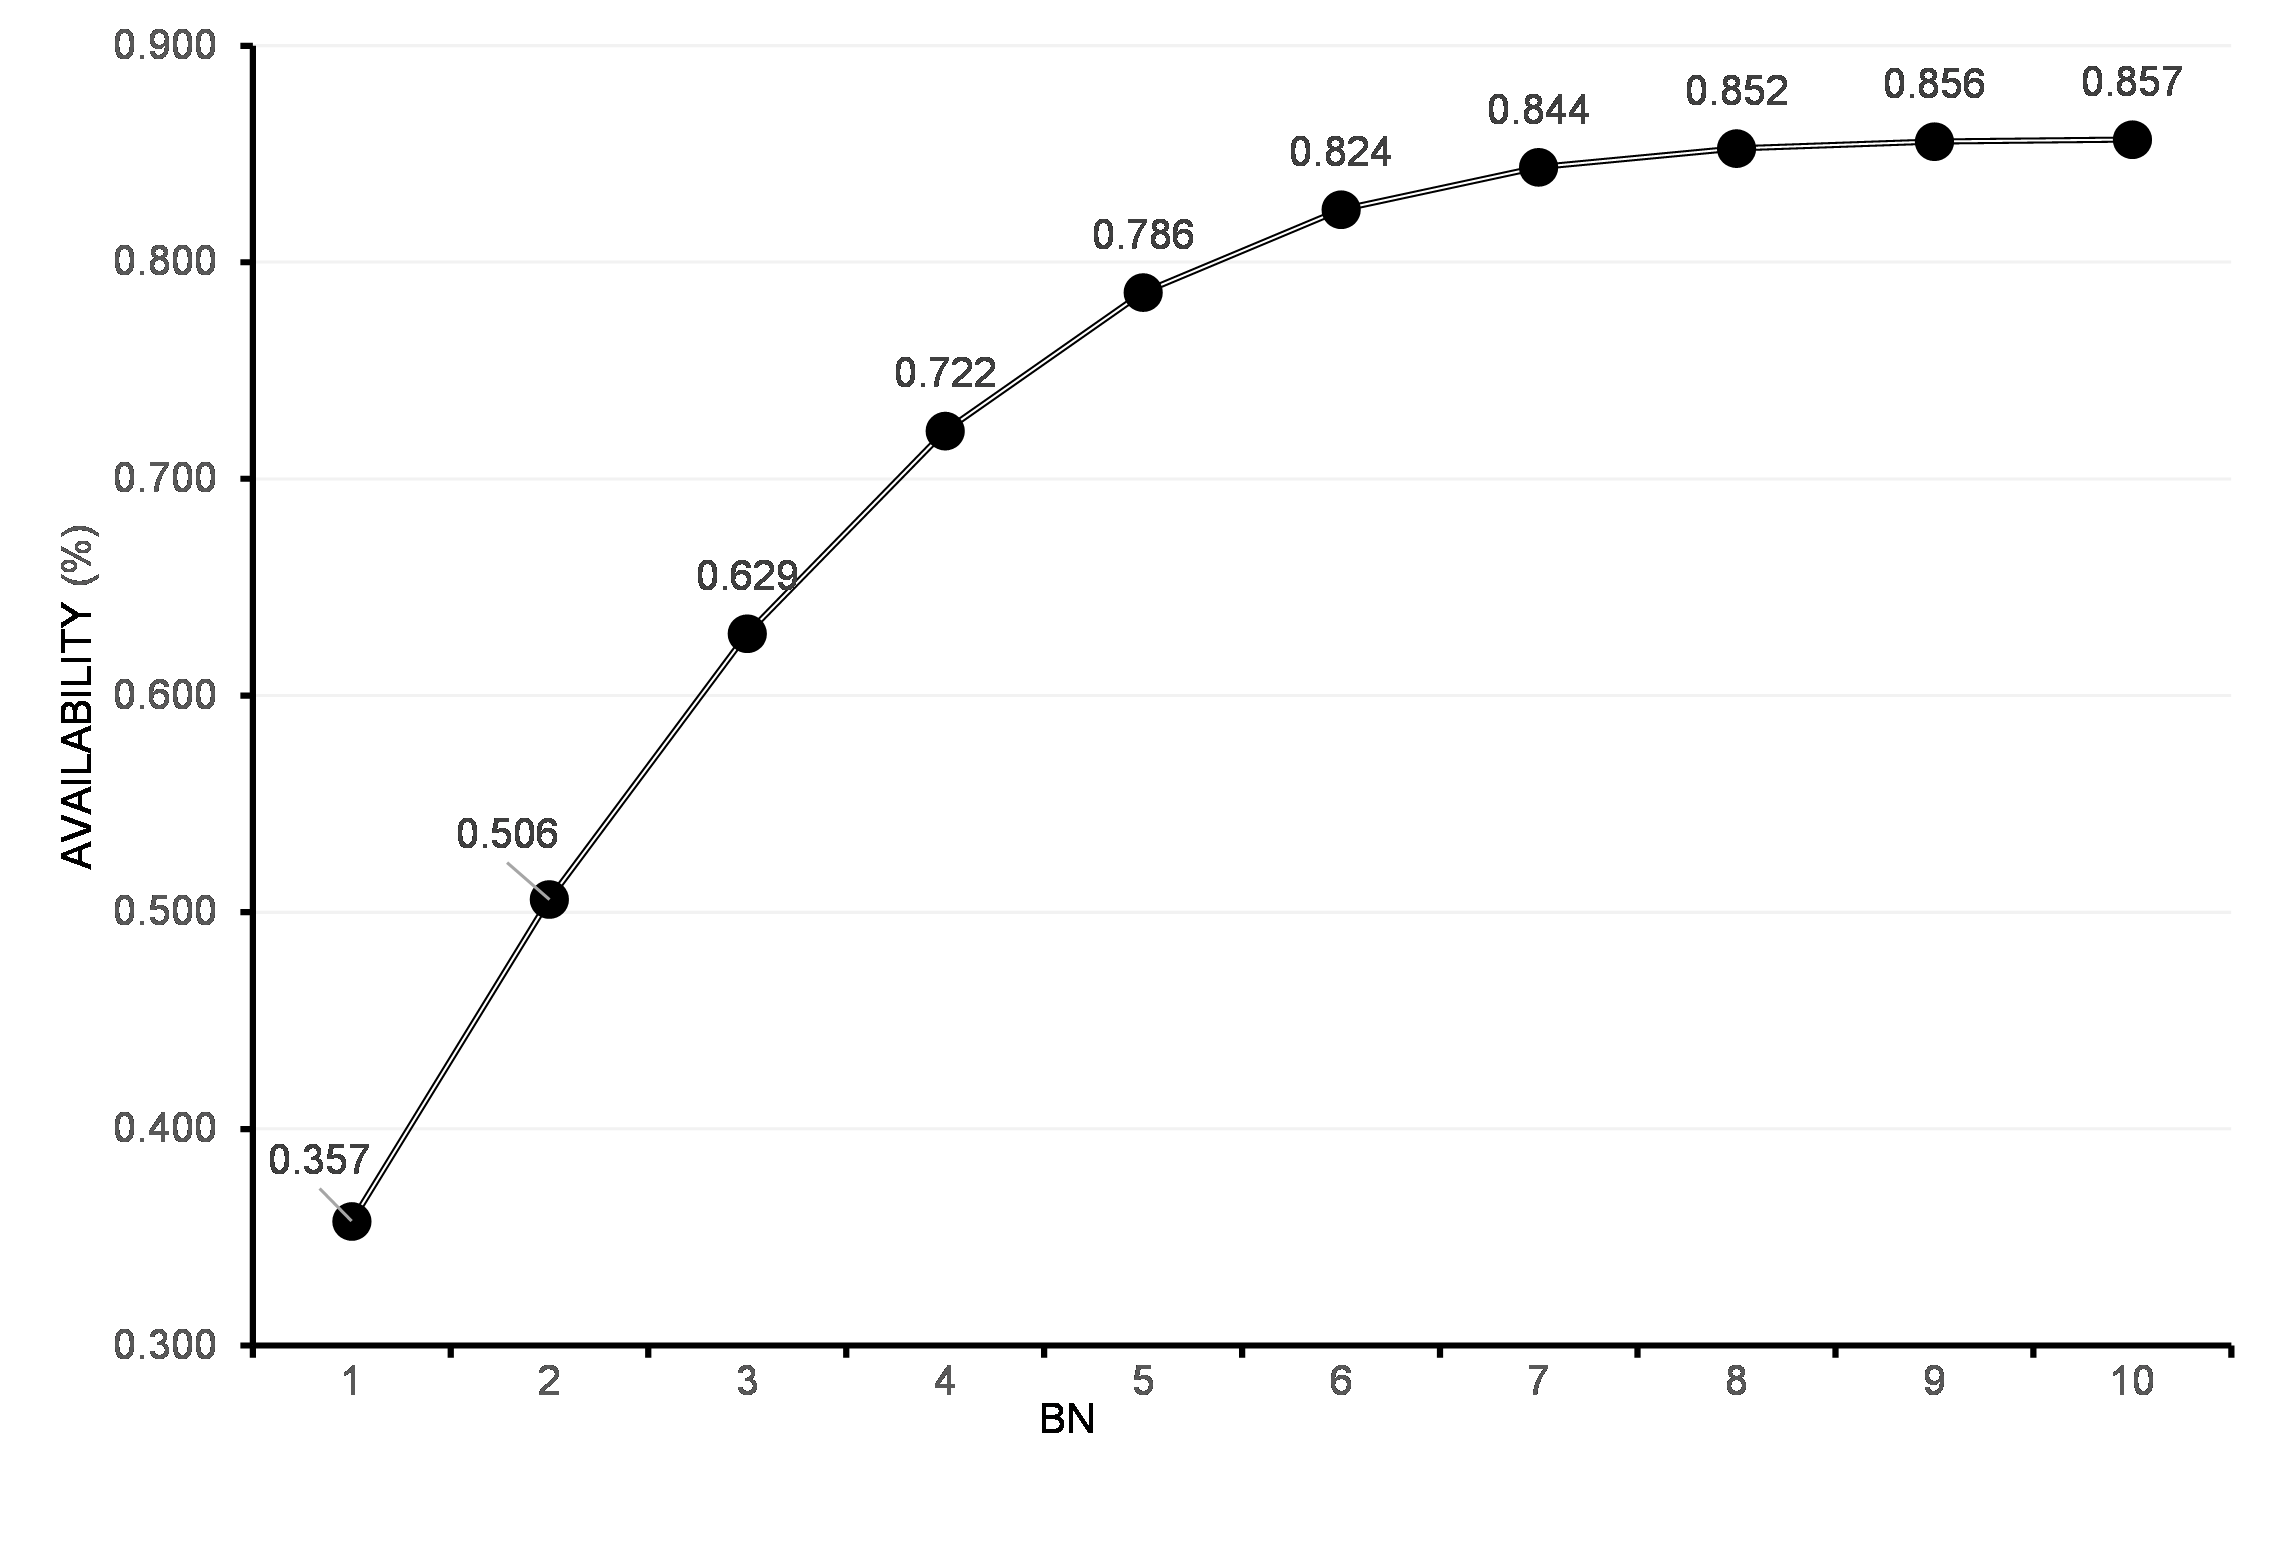
\includegraphics[scale=0.45]{img/exps/SA_006.png}}
\caption{Availability by number of batteries with basic operating mode MTT parameters}
\label{fig:basic_spn_sa_battery}
\end{figure}

\begin{figure}[htbp]
\centerline{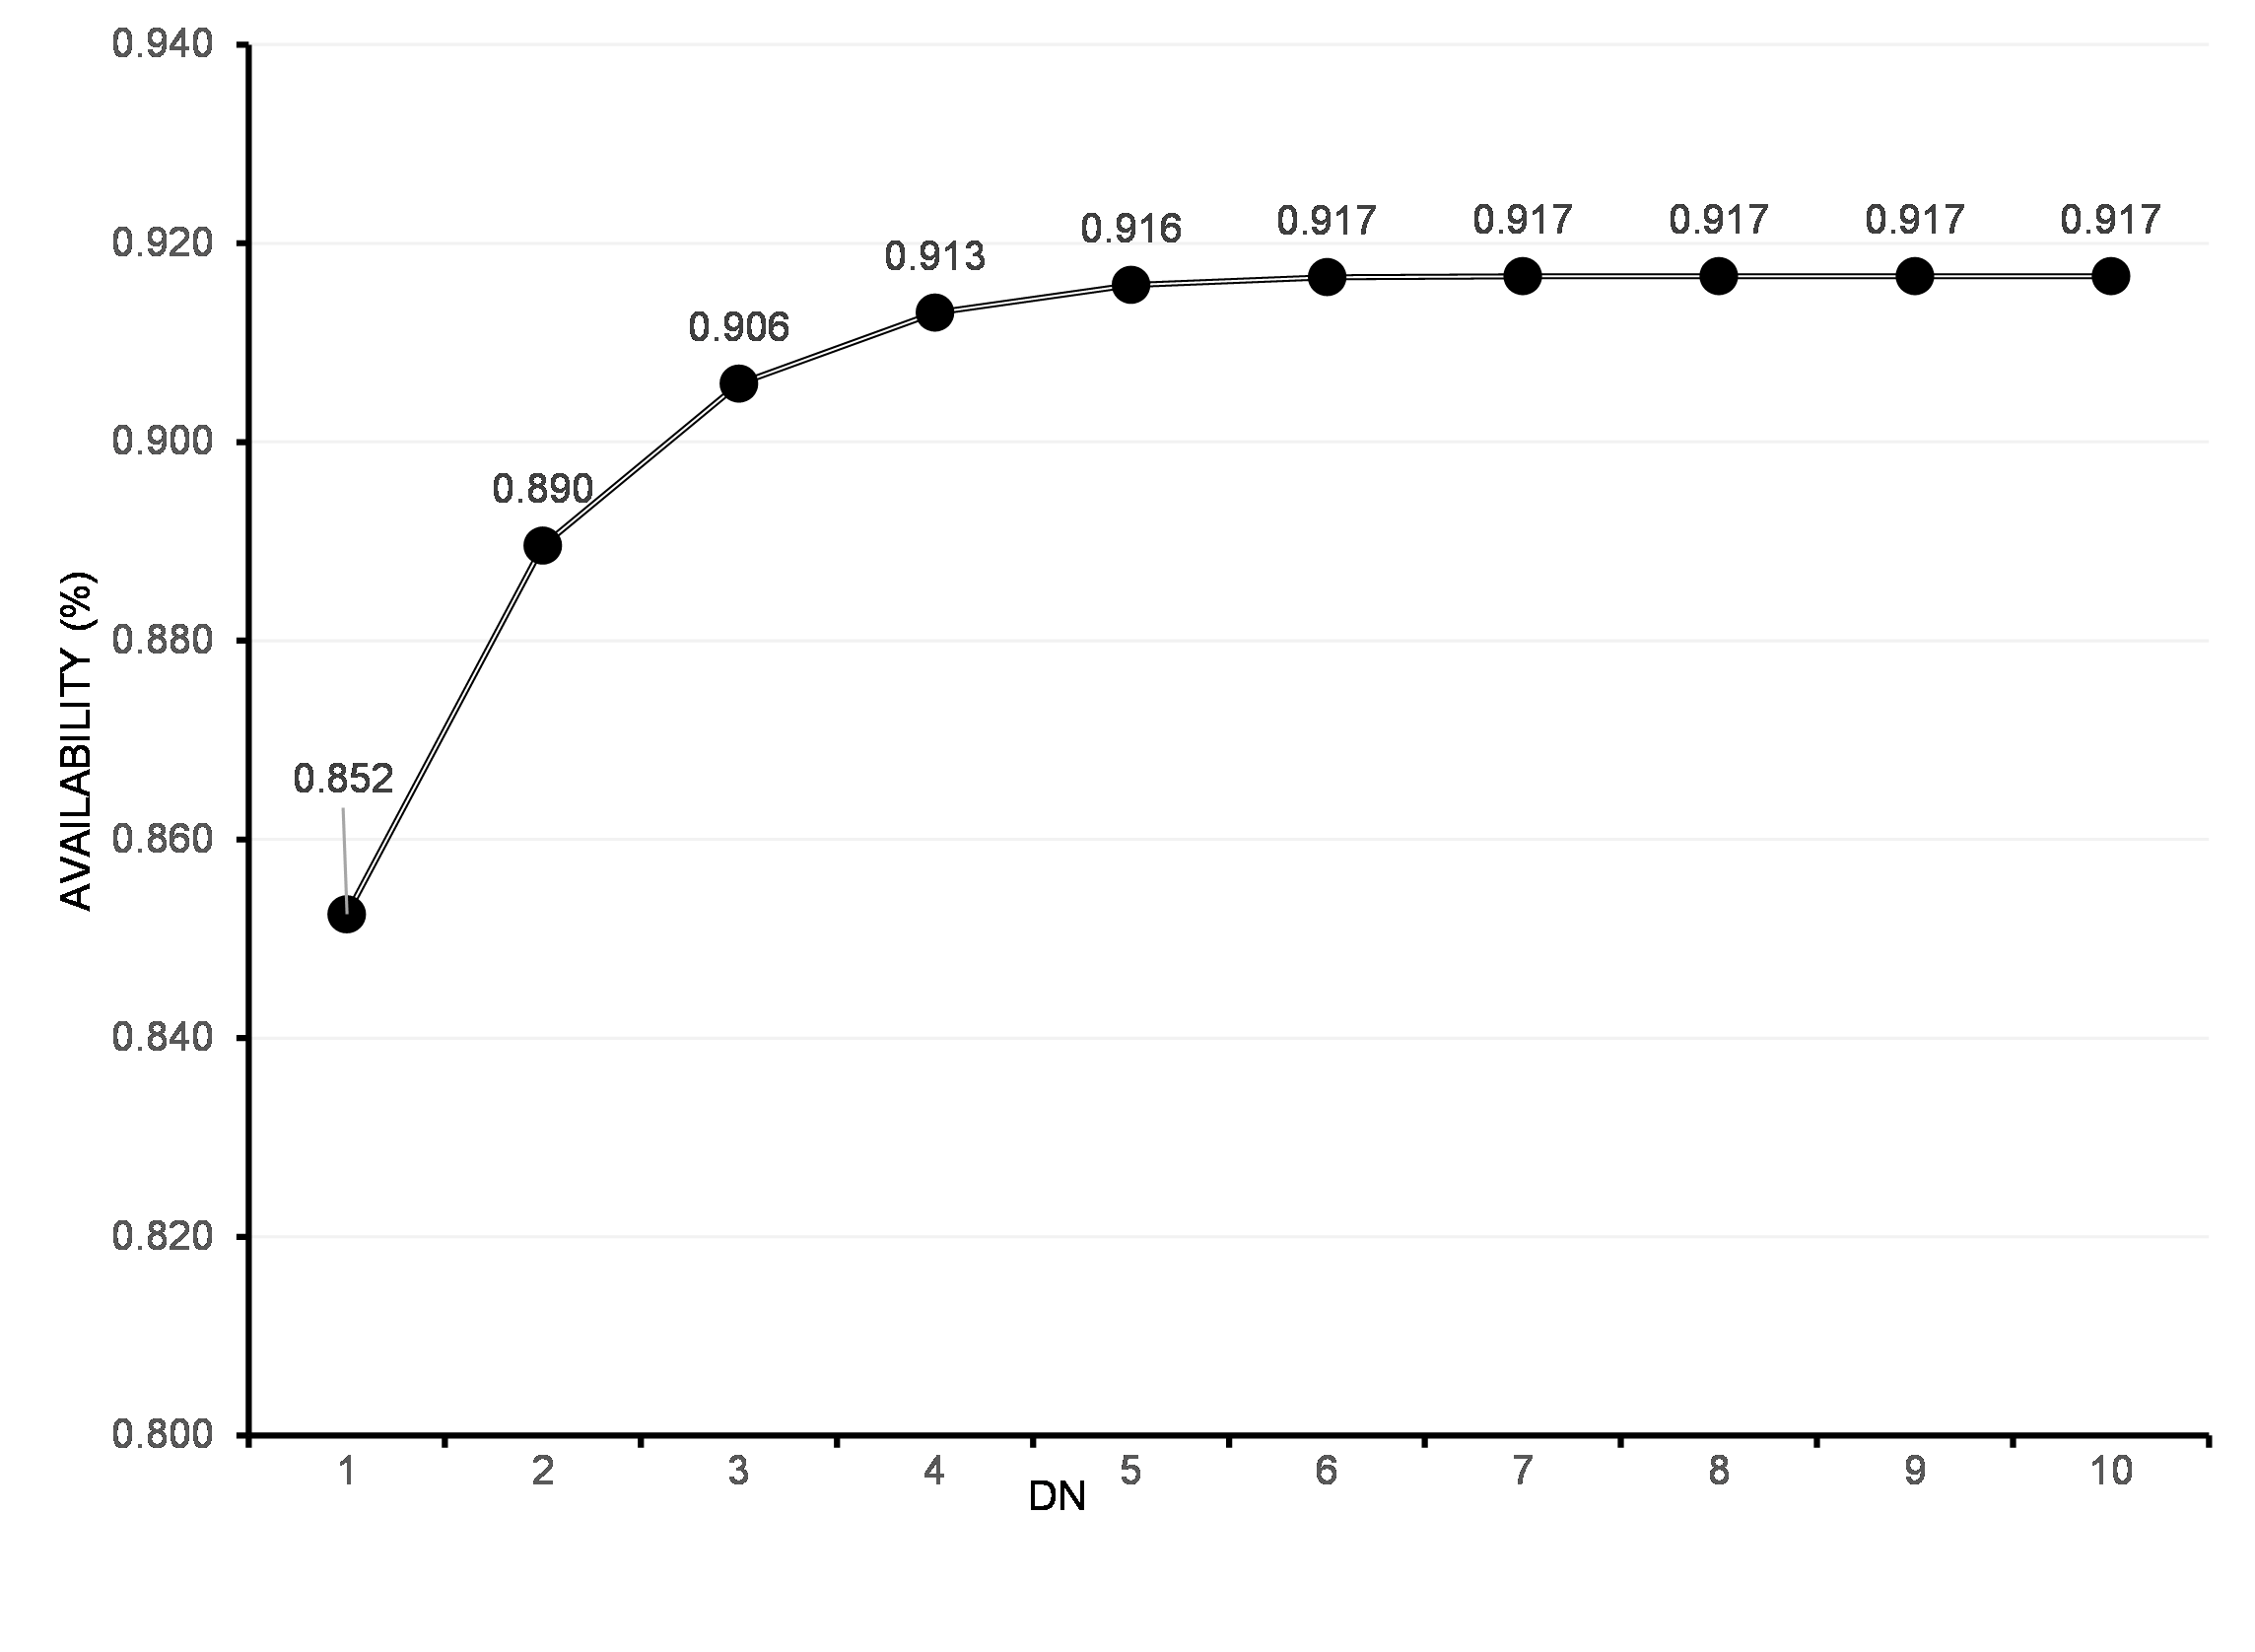
\includegraphics[scale=0.45]{img/exps/SA_003.png}}
\caption{Availability by number of UAVs with basic operating mode MTT parameters}
\label{fig:basic_spn_sa_uav}
\end{figure}


Figure \ref{fig:basic_spn_sa_battery} shows the evolution of the general availability of the system only with the application of redundancy in the battery component. We have an availability of 0.85\% using 8 spare batteries ready for use.

With the value of spare batteries (NB) set at 8, we vary the value of spare drones (ND) and obtain an availability of nine (0.90\%) with 4 spare drones (Fig. \ref{fig:basic_spn_sa_uav}) . However, we could not get availability with numbers of nines greater than 0.9\% just by adding redundancy mechanisms or isolated improvements to the baseline system.


\subsection{Case study 3}\label{sec:case_studies_sub03}

This third case study is a combination of the last two, in which we will evaluate the redundancy variations in the battery and UAV components using improved parameters from case study 1 to try to achieve availability greater than a nine. The enhanced parameter values that were used as input are defined in the \ref{tab:spn_parameter_values} table.

\begin{table}[htbp]
\caption{Improved parameter values for the SPN model}
\begin{center}
\begin{tabular}{|c|c|}
\hline
\textbf{\textit{Parameter}} & \textbf{\textit{Value (hours)}} \\
\hline
  MTTFD & 5000\\
 MTTRD & 2\\
 MTTBD & 2 \\ 
 MTTBC & 0.5 \\
 MTTSD & 0.016666667 \\
 NB & 1 \\
 ND & 1 \\
\hline
\end{tabular}
\label{tab:spn_parameter_values}
\end{center}
\end{table}

\begin{figure}[htbp]
\centerline{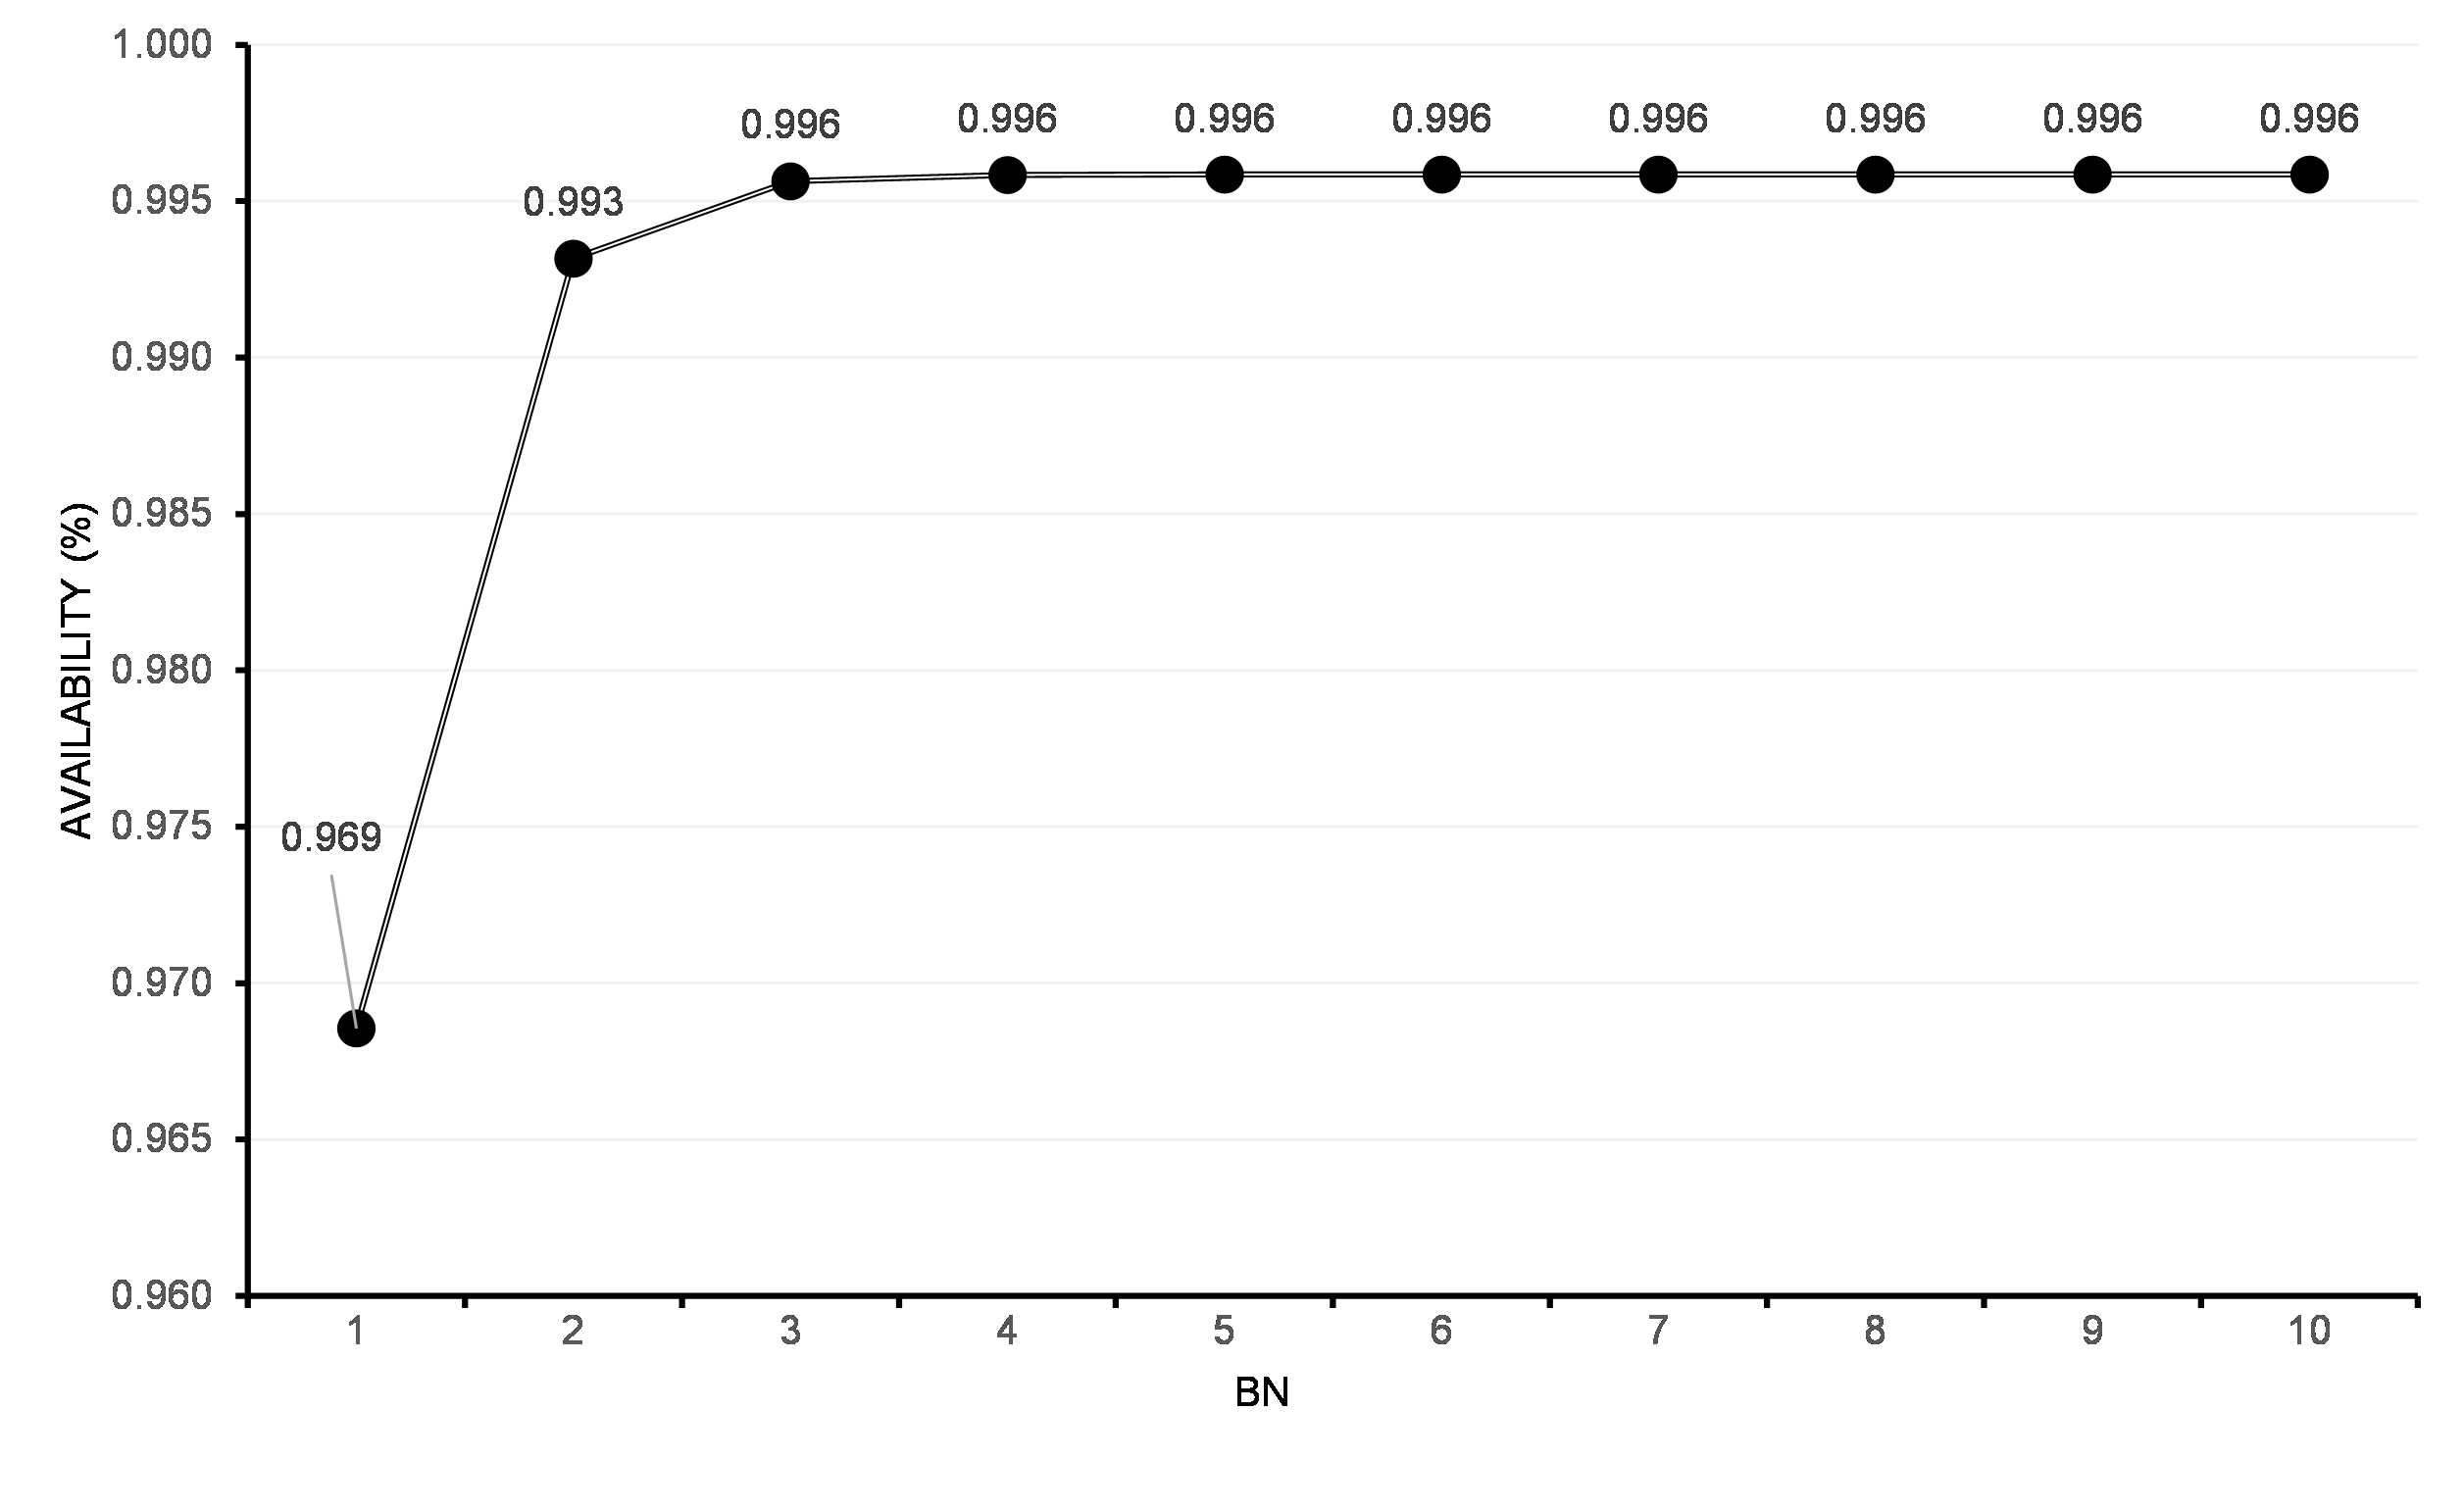
\includegraphics[scale=0.4]{img/exps/SA_005.png}}
\caption{Availability by number of batteries with improved MTT parameters}
\label{fig:spn_sa_battery}
\end{figure}


\begin{figure}[htbp]
\centerline{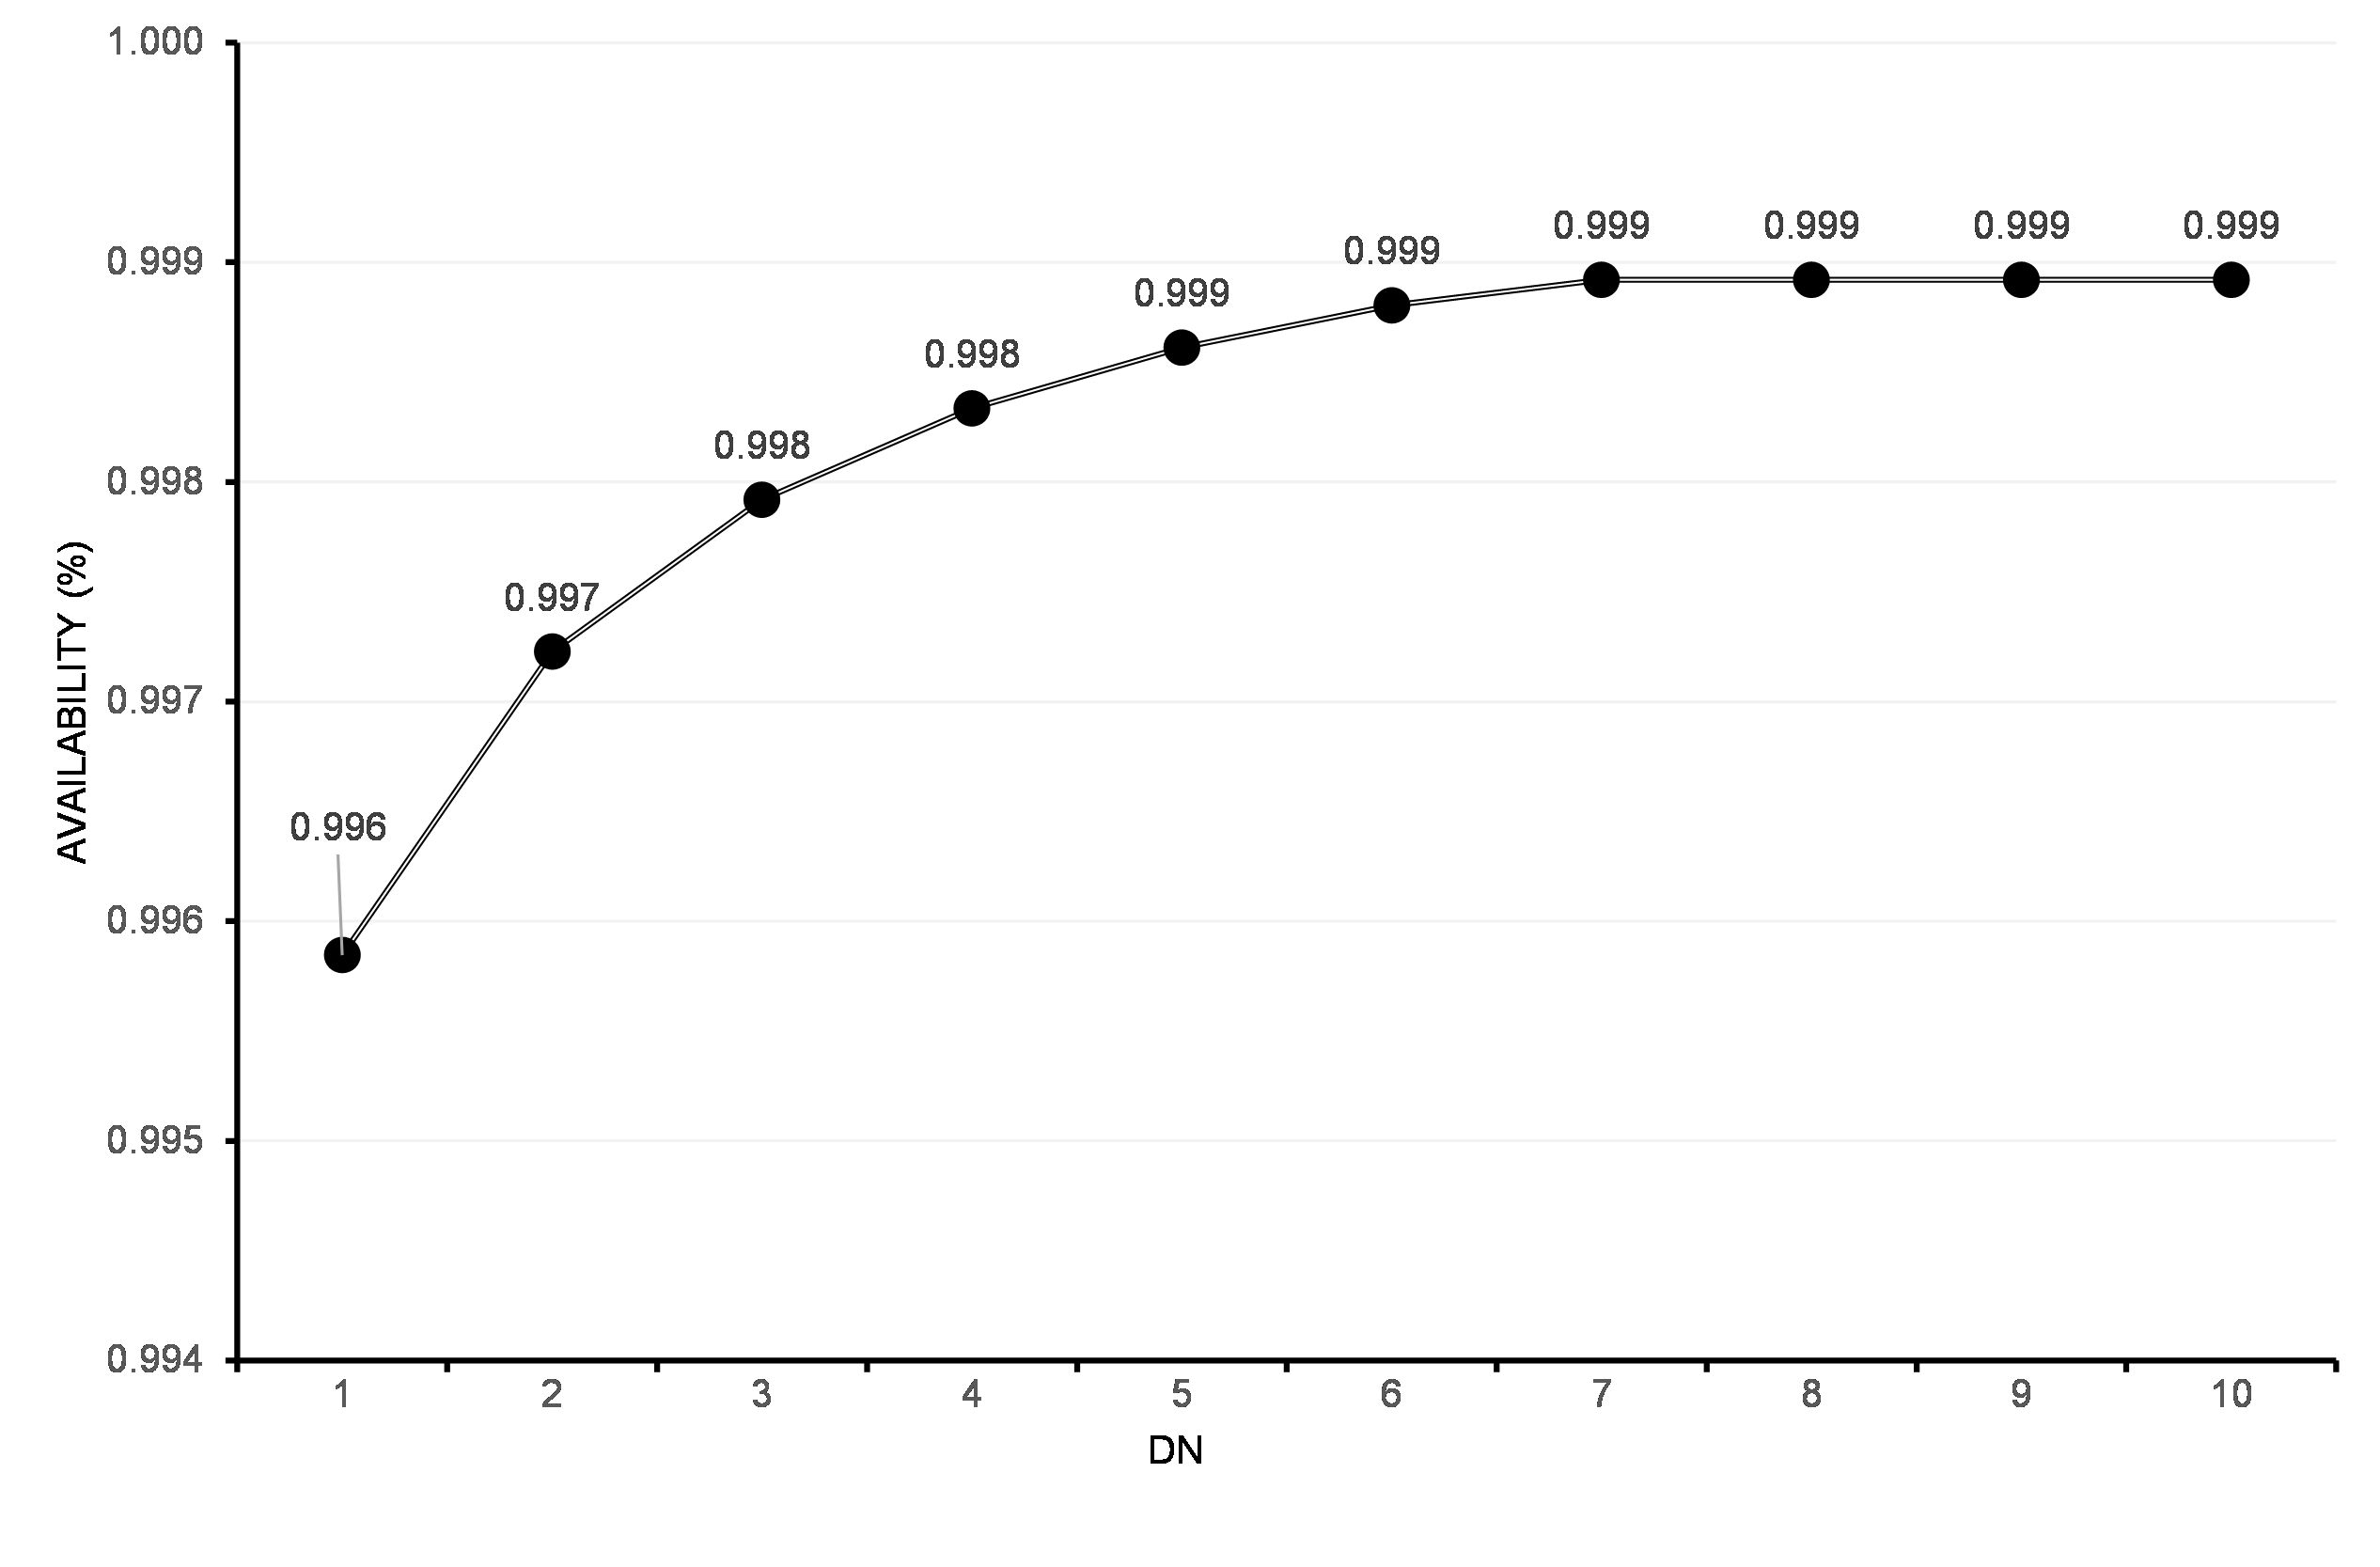
\includegraphics[scale=0.4]{img/exps/SA_004.png}}
\caption{Availability by number of UAVs with improved MTT parameters}
\label{fig:spn_sa_uav}
\end{figure}

At a first moment, we can see that we managed to obtain availability with a number of nines equal to 2 only with the addition of an extra battery (Fig.\ref{fig:spn_sa_battery}), with an initial availability of improved parameters from the study of case 1 of 0.97\%.

Finally, in Figure \ref{fig:spn_sa_uav}, we have the graph of variation in the use of extra UAVs devices for redundancy, reaching an availability of 3 nines (0.999\%) with the use of 4 extra UAVs. The use of fewer UAVs and spare batteries compared to the previous study can represent a considerable discount on the final budget of a system with these characteristics.


\section{Conclusions and future work}\label{sec:conclusions}

This work proposes two models for evaluating the availability of critical monitoring systems implemented in UAVs devices. In three case studies, an assessment of the availability of the system is carried out, given the improvements made and models used. 

The first case study varies baseline system time parameters symbolizing component improvements. The improvements had a limited availability of 0.97\%. In the second case study, with the same baseline, using redundancy mechanisms and a Petri net model, the availability improvement was limited to 0.91\% with 8 battery and 6 spare UAVs. Finally, in the last case study, we had a significant improvement in availability benefiting from improvements in the components with the joint use of redundancy mechanisms, which allowed an overall availability of the system in the house of 3 nines, 0.999\%.

As a future work, we intend to evaluate cost vs availability metrics of the case studies performed and perform an availability comparison of this type of system implemented in the cloud, fog and edge computing paradigms.


\section*{Acknowledgment}\label{sec:acknowledgment}
The authors would like to thank the Brazilian government for financial support through the Fundação de Amparo a Ciência e Tecnologia de Pernambuco (FACEPE), Modeling Distributed and Concurrent Systems (MoDCS) group for helping to improve this research.


\bibliographystyle{plainnat}
\bibliography{references}

\end{document}
